\documentclass[aspectratio=169,11pt]{beamer}

\usetheme{default}
\setbeamertemplate{navigation symbols}{}
\setbeamertemplate{footline}[frame number]
\usepackage{amsmath,amssymb}
\usepackage{tikz}
\usetikzlibrary{calc,decorations.pathreplacing,shapes.geometric,positioning}
\newcommand{\ct}{^{\mathsf H}}            % conjugate transpose
\usepackage{nicematrix}
\usepackage{algorithm}
\usepackage{algpseudocode}
\algrenewcommand\alglinenumber[1]{\scriptsize #1:}

% level colours (V_0, V_1, V_2)
\definecolor{lvlzero}{RGB}{200,60,60}
\definecolor{lvlone}{RGB}{40,120,60}
\definecolor{lvltwo}{RGB}{50,90,190}

% sparsity pictures of the solver steps
\colorlet{nz}{blue!25}      % nonzero block, unchanged w.r.t. T
\colorlet{mod}{orange!45}   % nonzero block, modified w.r.t. T
\colorlet{tri}{red!65}      % lower-triangular block that is solved
\colorlet{gone}{gray!30}    % rows/columns removed by deflation
\colorlet{grpA}{violet!35}  % merged node {1,2,5}
\colorlet{grpB}{teal!35}    % merged node {3,4,6}
% \vblk{x}{y}{height}{colour}{label}: one block of a vector, 6mm wide, top-left corner at (x,y)
\newcommand{\vblk}[5]{\fill[#4] (#1,#2) rectangle ++(6mm,-#3); \draw (#1,#2) rectangle ++(6mm,-#3);
  \node[font=\tiny] at ($(#1,#2)+(3mm,-0.5*#3)$) {#5};}
% \cell{a\\b}: a table cell with line breaks
\newcommand{\cell}[1]{\begin{tabular}[t]{@{}l@{}}#1\end{tabular}}
\newcommand{\swatch}[1]{\tikz\fill[#1,draw=black,line width=0.3pt] (0,0) rectangle (2mm,2mm);}

% \leafstep{1}: block pattern of T after diag(q_i^H) on the leaves 1,...,4
% \leafstep{2}: ... and after diag(w_i^H)
% \leafstep{3}: ... and with the solved rows and the z_i columns deflated
% Lines: thick = levels, solid = blocks, dashed = subdivision of a block.
\newcommand{\leafstep}[1]{%
\begin{tikzpicture}[x=6.5mm,y=-6.5mm]\leafpattern{#1}\end{tikzpicture}}
% \leafpattern{#1}: the drawing commands of \leafstep, for reuse in larger pictures
\newcommand{\leafpattern}[1]{%
\fill[nz] (0,0) rectangle (7,7);
\fill[mod] (0,0) rectangle (7,4);
\ifnum#1>1 \fill[mod] (0,0) rectangle (4,7); \fi
\foreach \i in {1,...,4} {\foreach \j in {1,...,7} {%
  \ifnum\i=\j\else\fill[white] (\j-1,\i-1) rectangle (\j,\i-0.5);\fi}}
\ifnum#1=2
\foreach \i in {1,...,4} {%
  \fill[white] (\i-1,\i-1) rectangle (\i,\i-0.5);
  \fill[tri] (\i-1,\i-1) -- (\i-1,\i-0.5) -- (\i-0.5,\i-0.5) -- cycle;}
\fi
\ifnum#1=3
\foreach \i in {1,...,4} {%
  \fill[gone] (0,\i-1) rectangle (7,\i-0.5);
  \fill[gone] (\i-1,0) rectangle (\i-0.5,7);}
\fi
\foreach \i in {1,...,4} \draw[dashed,line width=0.4pt] (0,\i-0.5) -- (7,\i-0.5);
\ifnum#1>1
\foreach \i in {1,...,4} \draw[dashed,line width=0.4pt] (\i-0.5,0) -- (\i-0.5,7);
\fi
\foreach \k in {1,...,6} \draw[line width=0.6pt] (\k,0) -- (\k,7) (0,\k) -- (7,\k);
\draw[line width=1.6pt] (0,0) rectangle (7,7);
\draw[line width=1.6pt] (4,0) -- (4,7) (6,0) -- (6,7) (0,4) -- (7,4) (0,6) -- (7,6);
\foreach \k in {1,...,7} {%
  \node[font=\scriptsize] at (\k-0.5,-0.35) {$\k$};
  \node[font=\scriptsize] at (-0.35,\k-0.5) {$\k$};}}

% The arbitrary tree of the notation slide (post-ordered, root 12), drawn radially:
% level l on the circle of radius 8l mm. The caller sets the styles tdot and tedge.
\newcommand{\radialtreebase}{%
\foreach \r in {8,16,24} \draw[gray!70,dashed] (0,0) circle (\r mm);
\node[tdot] (n12) at (0,0) {};
\node[tdot] (n5) at (150:8mm) {};
\node[tdot] (n10) at (30:8mm) {};
\node[tdot] (n11) at (270:8mm) {};
\foreach \k/\a in {1/105,2/135,3/165,4/195,9/30} \node[tdot] (n\k) at (\a:16mm) {};
\foreach \k/\a in {6/5,7/30,8/55} \node[tdot] (n\k) at (\a:24mm) {};
\draw[tedge] (n12) -- (n5) (n12) -- (n10) (n12) -- (n11) (n10) -- (n9);
\foreach \k in {1,2,3,4} \draw[tedge] (n5) -- (n\k);
\foreach \k in {6,7,8} \draw[tedge] (n9) -- (n\k);}

\title{TQS implicit ULV solver}
\date{}

\begin{document}

\begin{frame}
\titlepage
\end{frame}

\begin{frame}{Notation}
\begin{columns}[c]
\begin{column}{0.40\textwidth}
\centering
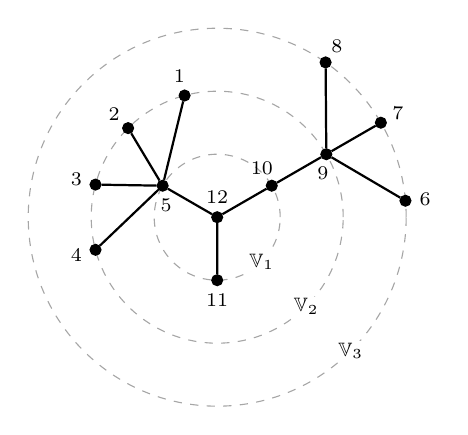
\begin{tikzpicture}[tdot/.style={circle,draw,fill=black,inner sep=1.4pt},tedge/.style={thick}]
\radialtreebase
% node labels: label of node k is placed at angle a, distance d from the node
\foreach \k/\a/\d in {12/90/2.5,5/280/2.5,10/120/2.5,11/270/2.5,9/-100/2.5,
                      1/105/2.5,2/135/2.5,3/165/2.5,4/195/2.5,6/5/2.5,7/30/2.5,8/55/2.5}
  \node[font=\scriptsize] at ($(n\k)+(\a:\d mm)$) {$\k$};
% level names on the circles
\foreach \l/\r in {1/8,2/16,3/24}
  \node[font=\scriptsize,fill=white,inner sep=0.5pt] at (-45:\r mm) {$\mathbb{V}_\l$};
\end{tikzpicture}

\vspace{2mm}
\scriptsize
$\mathbb{V}_0=\{12\}$, $\mathbb{V}_1=\{5,10,11\}$, $\mathbb{V}_2=\{1,2,3,4,9\}$, $\mathbb{V}_3=\{6,7,8\}$
\end{column}

\begin{column}{0.59\textwidth}
\footnotesize
\renewcommand{\arraystretch}{1.15}
\setlength{\tabcolsep}{4pt}
\begin{tabular}{@{}ll@{}}
\multicolumn{2}{@{}l}{\textbf{Tree}} \\
$r$ & root; here $r=12$ \\
$\mathbb{V}_\ell$ & level $\ell$: nodes at distance $\ell$ from $r$ \\
$L$ & depth; here $L=3$ \\
$\mathcal{P}(i)$ & parent of $i$, e.g.\ $\mathcal{P}(1)=5$, $\mathcal{P}(9)=10$ \\
$\mathcal{C}(i)$ & children of $i$, e.g.\ $\mathcal{C}(9)=\{6,7,8\}$, $\mathcal{C}(10)=\{9\}$ \\
leaf & node without children, e.g.\ $1$, $6$, $11$ \\[3pt]
\multicolumn{2}{@{}l}{\textbf{Matrix}} \\
$m_k$, $n_k$ & rows / columns of the block of node $k$ \\
$\rho_{i,j}$ & state dimension on the edge $i\to j$ \\
$\mathrm{T}(I,J)$ & block rows $I$, block columns $J$ of $\mathrm{T}$ \\
virtual & node $k$ with $m_k=n_k=0$ \\
$(\cdot)\ct$ & conjugate transpose \\
$\operatorname{diag}$, $\operatorname{blkdiag}$ & block-diagonal matrix of the arguments
\end{tabular}
\end{column}
\end{columns}

\end{frame}

\begin{frame}{The level-2 regular binary TQS matrix}
\begin{columns}[T]
\begin{column}{0.36\textwidth}
\centering
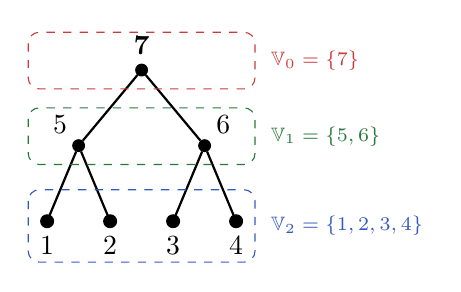
\begin{tikzpicture}[scale=0.8,
  level distance=12mm,
  level 1/.style={sibling distance=20mm},
  level 2/.style={sibling distance=10mm},
  every node/.style={circle,draw,fill=black,inner sep=1.5pt},
  edge from parent/.style={draw,thick}]
\node (n7) {}
  child { node (n5) {} child { node (n1) {} } child { node (n2) {} } }
  child { node (n6) {} child { node (n3) {} } child { node (n4) {} } };
\begin{scope}[every node/.style={}]
\node[above=2pt] at (n7) {$\mathbf{7}$};
\node[above left=1pt] at (n5) {$5$};
\node[above right=1pt] at (n6) {$6$};
\node[below=2pt] at (n1) {$1$};
\node[below=2pt] at (n2) {$2$};
\node[below=2pt] at (n3) {$3$};
\node[below=2pt] at (n4) {$4$};
\end{scope}
% boxes around the levels V_0, V_1, V_2
\begin{scope}[every node/.style={anchor=west,font=\scriptsize}]
\draw[lvlzero,dashed,rounded corners] (-18mm,6mm) rectangle (18mm,-3mm);
\node[lvlzero] at (19mm,1.5mm) {$\mathbb{V}_0=\{7\}$};
\draw[lvlone,dashed,rounded corners] (-18mm,-6mm) rectangle (18mm,-15mm);
\node[lvlone] at (19mm,-10.5mm) {$\mathbb{V}_1=\{5,6\}$};
\draw[lvltwo,dashed,rounded corners] (-18mm,-19mm) rectangle (18mm,-30.5mm);
\node[lvltwo] at (19mm,-24.75mm) {$\mathbb{V}_2=\{1,2,3,4\}$};
\end{scope}
\end{tikzpicture}

\vspace{2mm}
\raggedright
\scriptsize
\textbf{Path transition.} Nodes $j\neq k$ are joined by a unique path
$j=p_0-p_1-\cdots-p_\nu=k$ of length $\nu$. Its transition operator, from edge $(j,p_1)$ to edge $(p_{\nu-1},k)$, is
\[
\Phi_{k,j}:=\mathrm{Trans}^{p_{\nu-1}}_{k,p_{\nu-2}}\cdots\mathrm{Trans}^{p_1}_{p_2,j},
\]
with $\Phi_{k,j}:=I$ if $\nu=1$. Then
$\mathrm{T}_{k,j}=\mathrm{Out}^k_{p_{\nu-1}}\,\Phi_{k,j}\,\mathrm{Inp}^j_{p_1}$.
\end{column}

\begin{column}{0.62\textwidth}
\footnotesize
On the acyclic graph, node $k$ has four kinds of generators. Picking a root turns the graph into a
tree, and only then do the letters $\mathrm{B},\mathrm{P},\mathrm{U},\mathrm{V},\mathrm{W},\mathrm{C},\mathrm{Q}$
appear: they record the direction relative to the root.

\vspace{2mm}
\scriptsize
\renewcommand{\arraystretch}{1.3}
\setlength{\tabcolsep}{3pt}
\begin{tabular}{@{}llll@{}}
\hline
\textbf{Graph} & \textbf{Role} & \textbf{Rooted tree} & \textbf{Size} \\
\hline
$\mathrm{D}^k$ & input $\to$ output & $\mathrm{D}^k$ & $m_k \times n_k$ \\
$\mathrm{Inp}^k_j$ & input $\to$ edge $(k,j)$ &
  \cell{$\mathrm{B}^k_j$: $j$ parent\\ $\mathrm{P}^k_j$: $j$ child} & $\rho_{k,j} \times n_k$ \\
$\mathrm{Trans}^k_{i,j}$ & edge $(j,k)\to$ edge $(k,i)$ &
  \cell{$\mathrm{U}^k_{i,j}$: $j$ child, $i$ parent\\ $\mathrm{V}^k_{i,j}$: $j$, $i$ children\\ $\mathrm{W}^k_{i,j}$: $j$ parent, $i$ child} &
  $\rho_{k,i} \times \rho_{j,k}$ \\
$\mathrm{Out}^k_i$ & edge $(i,k)\to$ output &
  \cell{$\mathrm{C}^k_i$: $i$ child\\ $\mathrm{Q}^k_i$: $i$ parent} & $m_k \times \rho_{i,k}$ \\
\hline
\end{tabular}
\end{column}
\end{columns}
\end{frame}

\begin{frame}{The level-2 regular binary TQS matrix}
\centering
\fontsize{5.5}{6.5}\selectfont
\setlength{\arraycolsep}{1pt}
\[
\mathrm{T} =
\begin{bNiceArray}{cccc|cc|c}[first-row,first-col]
 & 1 & 2 & 3 & 4 & 5 & 6 & 7 \\[6pt]
1 & \mathrm{D}^{1} & \mathrm{Q}^{1}_{5}\mathrm{V}^{5}_{1,2}\mathrm{B}^{2}_{5} & \mathrm{Q}^{1}_{5}\mathrm{W}^{5}_{1,7}\mathrm{V}^{7}_{5,6}\mathrm{U}^{6}_{7,3}\mathrm{B}^{3}_{6} & \mathrm{Q}^{1}_{5}\mathrm{W}^{5}_{1,7}\mathrm{V}^{7}_{5,6}\mathrm{U}^{6}_{7,4}\mathrm{B}^{4}_{6} & \mathrm{Q}^{1}_{5}\mathrm{P}^{5}_{1} & \mathrm{Q}^{1}_{5}\mathrm{W}^{5}_{1,7}\mathrm{V}^{7}_{5,6}\mathrm{B}^{6}_{7} & \mathrm{Q}^{1}_{5}\mathrm{W}^{5}_{1,7}\mathrm{P}^{7}_{5} \\[6pt]
2 & \mathrm{Q}^{2}_{5}\mathrm{V}^{5}_{2,1}\mathrm{B}^{1}_{5} & \mathrm{D}^{2} & \mathrm{Q}^{2}_{5}\mathrm{W}^{5}_{2,7}\mathrm{V}^{7}_{5,6}\mathrm{U}^{6}_{7,3}\mathrm{B}^{3}_{6} & \mathrm{Q}^{2}_{5}\mathrm{W}^{5}_{2,7}\mathrm{V}^{7}_{5,6}\mathrm{U}^{6}_{7,4}\mathrm{B}^{4}_{6} & \mathrm{Q}^{2}_{5}\mathrm{P}^{5}_{2} & \mathrm{Q}^{2}_{5}\mathrm{W}^{5}_{2,7}\mathrm{V}^{7}_{5,6}\mathrm{B}^{6}_{7} & \mathrm{Q}^{2}_{5}\mathrm{W}^{5}_{2,7}\mathrm{P}^{7}_{5} \\[6pt]
3 & \mathrm{Q}^{3}_{6}\mathrm{W}^{6}_{3,7}\mathrm{V}^{7}_{6,5}\mathrm{U}^{5}_{7,1}\mathrm{B}^{1}_{5} & \mathrm{Q}^{3}_{6}\mathrm{W}^{6}_{3,7}\mathrm{V}^{7}_{6,5}\mathrm{U}^{5}_{7,2}\mathrm{B}^{2}_{5} & \mathrm{D}^{3} & \mathrm{Q}^{3}_{6}\mathrm{V}^{6}_{3,4}\mathrm{B}^{4}_{6} & \mathrm{Q}^{3}_{6}\mathrm{W}^{6}_{3,7}\mathrm{V}^{7}_{6,5}\mathrm{B}^{5}_{7} & \mathrm{Q}^{3}_{6}\mathrm{P}^{6}_{3} & \mathrm{Q}^{3}_{6}\mathrm{W}^{6}_{3,7}\mathrm{P}^{7}_{6} \\[6pt]
4 & \mathrm{Q}^{4}_{6}\mathrm{W}^{6}_{4,7}\mathrm{V}^{7}_{6,5}\mathrm{U}^{5}_{7,1}\mathrm{B}^{1}_{5} & \mathrm{Q}^{4}_{6}\mathrm{W}^{6}_{4,7}\mathrm{V}^{7}_{6,5}\mathrm{U}^{5}_{7,2}\mathrm{B}^{2}_{5} & \mathrm{Q}^{4}_{6}\mathrm{V}^{6}_{4,3}\mathrm{B}^{3}_{6} & \mathrm{D}^{4} & \mathrm{Q}^{4}_{6}\mathrm{W}^{6}_{4,7}\mathrm{V}^{7}_{6,5}\mathrm{B}^{5}_{7} & \mathrm{Q}^{4}_{6}\mathrm{P}^{6}_{4} & \mathrm{Q}^{4}_{6}\mathrm{W}^{6}_{4,7}\mathrm{P}^{7}_{6} \\[6pt]
\hline
5 & \mathrm{C}^{5}_{1}\mathrm{B}^{1}_{5} & \mathrm{C}^{5}_{2}\mathrm{B}^{2}_{5} & \mathrm{Q}^{5}_{7}\mathrm{V}^{7}_{5,6}\mathrm{U}^{6}_{7,3}\mathrm{B}^{3}_{6} & \mathrm{Q}^{5}_{7}\mathrm{V}^{7}_{5,6}\mathrm{U}^{6}_{7,4}\mathrm{B}^{4}_{6} & \mathrm{D}^{5} & \mathrm{Q}^{5}_{7}\mathrm{V}^{7}_{5,6}\mathrm{B}^{6}_{7} & \mathrm{Q}^{5}_{7}\mathrm{P}^{7}_{5} \\[6pt]
6 & \mathrm{Q}^{6}_{7}\mathrm{V}^{7}_{6,5}\mathrm{U}^{5}_{7,1}\mathrm{B}^{1}_{5} & \mathrm{Q}^{6}_{7}\mathrm{V}^{7}_{6,5}\mathrm{U}^{5}_{7,2}\mathrm{B}^{2}_{5} & \mathrm{C}^{6}_{3}\mathrm{B}^{3}_{6} & \mathrm{C}^{6}_{4}\mathrm{B}^{4}_{6} & \mathrm{Q}^{6}_{7}\mathrm{V}^{7}_{6,5}\mathrm{B}^{5}_{7} & \mathrm{D}^{6} & \mathrm{Q}^{6}_{7}\mathrm{P}^{7}_{6} \\[6pt]
\hline
7 & \mathrm{C}^{7}_{5}\mathrm{U}^{5}_{7,1}\mathrm{B}^{1}_{5} & \mathrm{C}^{7}_{5}\mathrm{U}^{5}_{7,2}\mathrm{B}^{2}_{5} & \mathrm{C}^{7}_{6}\mathrm{U}^{6}_{7,3}\mathrm{B}^{3}_{6} & \mathrm{C}^{7}_{6}\mathrm{U}^{6}_{7,4}\mathrm{B}^{4}_{6} & \mathrm{C}^{7}_{5}\mathrm{B}^{5}_{7} & \mathrm{C}^{7}_{6}\mathrm{B}^{6}_{7} & \mathrm{D}^{7}
\CodeAfter
  \begin{tikzpicture}[decoration={brace,amplitude=3pt},font=\scriptsize]
  % row blocks (right)
  \draw[lvltwo,thick,decorate] ([xshift=4mm]1-|8) -- ([xshift=4mm]5-|8)
    node[midway,right=3pt] {$\mathbb{V}_2$};
  \draw[lvlone,thick,decorate] ([xshift=4mm]5-|8) -- ([xshift=4mm]7-|8)
    node[midway,right=3pt] {$\mathbb{V}_1$};
  \draw[lvlzero,thick,decorate] ([xshift=4mm]7-|8) -- ([xshift=4mm]8-|8)
    node[midway,right=3pt] {$\mathbb{V}_0$};
  % column blocks (below)
  \draw[lvltwo,thick,decorate] ([yshift=-2mm]8-|5) -- ([yshift=-2mm]8-|1)
    node[midway,below=3pt] {$\mathbb{V}_2$};
  \draw[lvlone,thick,decorate] ([yshift=-2mm]8-|7) -- ([yshift=-2mm]8-|5)
    node[midway,below=3pt] {$\mathbb{V}_1$};
  \draw[lvlzero,thick,decorate] ([yshift=-2mm]8-|8) -- ([yshift=-2mm]8-|7)
    node[midway,below=3pt] {$\mathbb{V}_0$};
  \end{tikzpicture}
\end{bNiceArray}
\]
\end{frame}

\begin{frame}{The diagonal blocks are HSS matrices}
\begin{columns}[c]
\begin{column}{0.40\textwidth}
\centering
% block partition of T, 6mm per node, rows/columns ordered 1,...,7
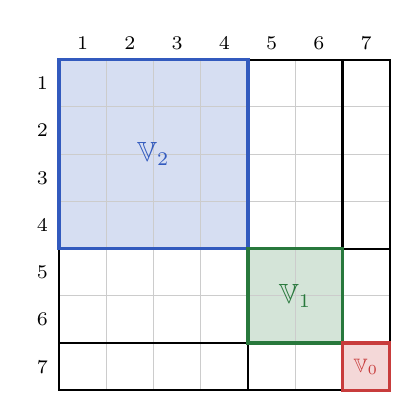
\begin{tikzpicture}[x=6mm,y=-6mm]
\fill[lvltwo!20]  (0,0) rectangle (4,4);
\fill[lvlone!20]  (4,4) rectangle (6,6);
\fill[lvlzero!20] (6,6) rectangle (7,7);
\foreach \k in {1,...,6} \draw[gray!40] (\k,0) -- (\k,7) (0,\k) -- (7,\k);
\draw[thick] (0,0) rectangle (7,7);
\draw[thick] (4,0) -- (4,7) (6,0) -- (6,7) (0,4) -- (7,4) (0,6) -- (7,6);
\draw[lvltwo,very thick]  (0,0) rectangle (4,4);
\draw[lvlone,very thick]  (4,4) rectangle (6,6);
\draw[lvlzero,very thick] (6,6) rectangle (7,7);
\foreach \k in {1,...,7} {
  \node[font=\scriptsize] at (\k-0.5,-0.35) {$\k$};
  \node[font=\scriptsize] at (-0.35,\k-0.5) {$\k$};
}
\node[lvltwo]  at (2,2)     {$\mathbb{V}_2$};
\node[lvlone]  at (5,5)     {$\mathbb{V}_1$};
\node[lvlzero,font=\scriptsize] at (6.5,6.5) {$\mathbb{V}_0$};
\end{tikzpicture}
\end{column}

\begin{column}{0.58\textwidth}
\footnotesize
\tikzset{
  mini/.style={level distance=5mm,
    every node/.style={circle,draw,inner sep=1.2pt},
    edge from parent/.style={draw}},
  virt/.style={fill=white},
}
\renewcommand{\arraystretch}{1.2}
\begin{tabular}{@{}c@{\quad}l@{}}
\begin{tikzpicture}[mini,baseline=-6mm,
  level 1/.style={sibling distance=10mm},level 2/.style={sibling distance=5mm}]
\node[virt] {}
  child { node[virt] {} child { node[fill=lvltwo] {} } child { node[fill=lvltwo] {} } }
  child { node[virt] {} child { node[fill=lvltwo] {} } child { node[fill=lvltwo] {} } };
\end{tikzpicture}
& \parbox[c]{0.68\linewidth}{\color{lvltwo}$\mathrm{T}(\mathbb{V}_2,\mathbb{V}_2)$: \textbf{level-2 HSS}\\[1pt]
  \color{black} leaves $1,2,3,4$; nodes $5,6,7$ are virtual} \\[6mm]
\begin{tikzpicture}[mini,baseline=-3mm,level 1/.style={sibling distance=6mm}]
\node[virt] {} child { node[fill=lvlone] {} } child { node[fill=lvlone] {} };
\end{tikzpicture}
& \parbox[c]{0.68\linewidth}{\color{lvlone}$\mathrm{T}(\mathbb{V}_1,\mathbb{V}_1)$: \textbf{level-1 HSS}\\[1pt]
  \color{black}$\begin{bmatrix} \mathrm{D}^5 & \mathrm{Q}^5_7\mathrm{V}^7_{5,6}\mathrm{B}^6_7 \\
  \mathrm{Q}^6_7\mathrm{V}^7_{6,5}\mathrm{B}^5_7 & \mathrm{D}^6 \end{bmatrix}$, node $7$ virtual} \\[6mm]
\begin{tikzpicture}[mini,baseline=-0.6mm]
\node[fill=lvlzero] {};
\end{tikzpicture}
& \parbox[c]{0.68\linewidth}{\color{lvlzero}$\mathrm{T}(\mathbb{V}_0,\mathbb{V}_0)=\mathrm{D}^7$: \textbf{level-0 HSS}}
\end{tabular}
\end{column}
\end{columns}

\vspace{4mm}
\begin{block}{Degeneration to HSS}
If every node outside $\mathbb{V}_i$ is \emph{virtual}, i.e.\ $m_k=n_k=0$ for all $k\notin\mathbb{V}_i$,
then $\mathrm{T}=\mathrm{T}(\mathbb{V}_i,\mathbb{V}_i)$ is a level-$i$ HSS matrix, $i=0,1,2$.
\end{block}
\end{frame}

\begin{frame}{The outer level: a 3-node SQS matrix}
\begin{columns}[c]
\begin{column}{0.36\textwidth}
\centering
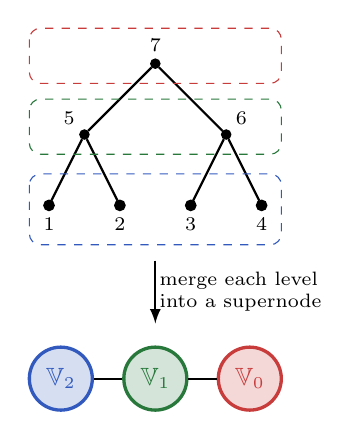
\begin{tikzpicture}[
  level distance=9mm,
  level 1/.style={sibling distance=18mm},
  level 2/.style={sibling distance=9mm},
  every node/.style={circle,draw,fill=black,inner sep=1.2pt},
  edge from parent/.style={draw,thick}]
\node (n7) {}
  child { node (n5) {} child { node (n1) {} } child { node (n2) {} } }
  child { node (n6) {} child { node (n3) {} } child { node (n4) {} } };
\begin{scope}[every node/.style={font=\scriptsize}]
\node[above=1pt] at (n7) {$7$};
\node[above left=0pt] at (n5) {$5$};
\node[above right=0pt] at (n6) {$6$};
\foreach \k in {1,2,3,4} \node[below=1pt] at (n\k) {$\k$};
\end{scope}
\draw[lvlzero,dashed,rounded corners] (-16mm,4.5mm) rectangle (16mm,-2.5mm);
\draw[lvlone,dashed,rounded corners] (-16mm,-4.5mm) rectangle (16mm,-11.5mm);
\draw[lvltwo,dashed,rounded corners] (-16mm,-14mm) rectangle (16mm,-23mm);
% merge into supernodes
\draw[-latex,thick] (0,-25mm) -- node[right,rectangle,draw=none,fill=none,font=\scriptsize,align=left]
  {merge each level\\into a supernode} (0,-33mm);
\begin{scope}[every node/.style={circle,draw,very thick,minimum size=8mm,font=\small}]
\node[lvltwo,fill=lvltwo!20]   (s2) at (-12mm,-40mm) {$\mathbb{V}_2$};
\node[lvlone,fill=lvlone!20]   (s1) at (0mm,-40mm)   {$\mathbb{V}_1$};
\node[lvlzero,fill=lvlzero!20] (s0) at (12mm,-40mm)  {$\mathbb{V}_0$};
\end{scope}
\draw[thick] (s2) -- (s1) -- (s0);
\end{tikzpicture}
\end{column}

\begin{column}{0.62\textwidth}
\footnotesize
Order the supernodes $[2]{=}\mathbb{V}_2,\ [1]{=}\mathbb{V}_1,\ [0]{=}\mathbb{V}_0$ on a line (root $[0]$).
Then $\mathrm{T}$ is a \textbf{3-node SQS matrix}:
\[
\mathrm{T}=
\begin{bmatrix}
\mathrm{D}^{[2]} & \mathrm{Q}^{[2]}_{[1]}\mathrm{P}^{[1]}_{[2]} & \mathrm{Q}^{[2]}_{[1]}\mathrm{W}^{[1]}_{[2],[0]}\mathrm{P}^{[0]}_{[1]} \\[2pt]
\mathrm{C}^{[1]}_{[2]}\mathrm{B}^{[2]}_{[1]} & \mathrm{D}^{[1]} & \mathrm{Q}^{[1]}_{[0]}\mathrm{P}^{[0]}_{[1]} \\[2pt]
\mathrm{C}^{[0]}_{[1]}\mathrm{U}^{[1]}_{[0],[2]}\mathrm{B}^{[2]}_{[1]} & \mathrm{C}^{[0]}_{[1]}\mathrm{B}^{[1]}_{[0]} & \mathrm{D}^{[0]}
\end{bmatrix}
\]
\begin{itemize}
\item Diagonal: $\mathrm{D}^{[\ell]}=\mathrm{T}(\mathbb{V}_\ell,\mathbb{V}_\ell)$, the HSS blocks of the previous slide.
\item States: supernode edge $[2]\to[1]$ carries the states on the tree edges
  $1{\to}5,\ 2{\to}5,\ 3{\to}6,\ 4{\to}6$:
  \[ \rho_{[2],[1]}=\rho_{1,5}+\rho_{2,5}+\rho_{3,6}+\rho_{4,6},
     \qquad \rho_{[1],[0]}=\rho_{5,7}+\rho_{6,7}, \]
  and likewise in the opposite direction.
\item E.g.\ $\mathrm{B}^{[2]}_{[1]}=\operatorname{blkdiag}(\mathrm{B}^1_5,\mathrm{B}^2_5,\mathrm{B}^3_6,\mathrm{B}^4_6)$.
\end{itemize}
\end{column}
\end{columns}
\end{frame}

\begin{frame}{Any leaf-to-root path gives a 3-node SQS matrix}
\begin{columns}[c]
\begin{column}{0.36\textwidth}
\centering
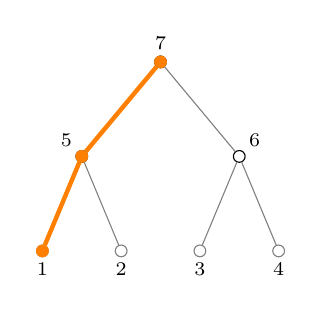
\begin{tikzpicture}[
  level distance=12mm,
  level 1/.style={sibling distance=20mm},
  level 2/.style={sibling distance=10mm},
  every node/.style={circle,draw,fill=white,inner sep=1.5pt},
  edge from parent/.style={draw,gray}]
\node (n7) {}
  child { node (n5) {} child { node (n1) {} } child { node (n2) {} } }
  child { node (n6) {} child { node (n3) {} } child { node (n4) {} } };
\draw[orange,ultra thick] (n1) -- (n5) -- (n7);
\foreach \k in {1,5,7} \node[fill=orange,draw=orange] at (n\k) {};
\begin{scope}[every node/.style={font=\scriptsize}]
\node[above=1pt] at (n7) {$7$};
\node[above left=0pt] at (n5) {$5$};
\node[above right=0pt] at (n6) {$6$};
\foreach \k in {1,2,3,4} \node[below=1pt] at (n\k) {$\k$};
\end{scope}
\end{tikzpicture}

\vspace{3mm}
\scriptsize
\tikz\node[circle,draw=orange,fill=orange,inner sep=1.5pt]{}; on the path \quad
\tikz\node[circle,draw,inner sep=1.5pt]{}; virtual
\end{column}

\begin{column}{0.62\textwidth}
\footnotesize
Take the path $1\to5\to7$ and set $m_k=n_k=0$ for all $k\notin\{1,5,7\}$. Then
\[
\mathrm{T}=
\begin{bmatrix}
\mathrm{D}^{1} & \mathrm{Q}^{1}_{5}\mathrm{P}^{5}_{1} & \mathrm{Q}^{1}_{5}\mathrm{W}^{5}_{1,7}\mathrm{P}^{7}_{5} \\[2pt]
\mathrm{C}^{5}_{1}\mathrm{B}^{1}_{5} & \mathrm{D}^{5} & \mathrm{Q}^{5}_{7}\mathrm{P}^{7}_{5} \\[2pt]
\mathrm{C}^{7}_{5}\mathrm{U}^{5}_{7,1}\mathrm{B}^{1}_{5} & \mathrm{C}^{7}_{5}\mathrm{B}^{5}_{7} & \mathrm{D}^{7}
\end{bmatrix},
\]
which is exactly the \textbf{3-node SQS matrix} on the line $1 - 5 - 7$ with root $7$.

\vspace{3mm}
The same holds for each of the four leaf-to-root paths
$1\to5\to7$, $2\to5\to7$, $3\to6\to7$, $4\to6\to7$.
\end{column}
\end{columns}
\end{frame}

\begin{frame}{Generalization: regular binary tree of depth $L$}
\footnotesize
\textbf{Setting.} Root $r$ at level $0$; level $\mathbb{V}_\ell$ has $2^\ell$ nodes, $\ell=0,\dots,L$;
$\mathrm{T}$ is ordered by levels $\mathbb{V}_L,\mathbb{V}_{L-1},\dots,\mathbb{V}_0$.

\vspace{3mm}
\begin{enumerate}
\setlength{\itemsep}{2mm}
\item \textbf{Diagonal blocks are HSS.} $\mathrm{T}(\mathbb{V}_\ell,\mathbb{V}_\ell)$ is a level-$\ell$ HSS matrix,
  $\ell=0,\dots,L$, with the nodes in $\mathbb{V}_0,\dots,\mathbb{V}_{\ell-1}$ acting as virtual nodes.
\item \textbf{Level degeneration.} If $m_k=n_k=0$ for all $k\notin\mathbb{V}_\ell$,
  then $\mathrm{T}$ is a level-$\ell$ HSS matrix.
\item \textbf{Outer level is SQS.} Merging each $\mathbb{V}_\ell$ into a supernode $[\ell]$, $\mathrm{T}$ is an
  $(L+1)$-node SQS matrix on the line $[L] - [L-1] - \cdots - [0]$. The state between $[\ell]$ and $[\ell-1]$
  collects the states on all tree edges between $\mathbb{V}_\ell$ and $\mathbb{V}_{\ell-1}$:
  \[ \rho_{[\ell],[\ell-1]}=\sum_{i\in\mathbb{V}_\ell}\rho_{i,\mathcal{P}(i)},
     \qquad \rho_{[\ell-1],[\ell]}=\sum_{i\in\mathbb{V}_\ell}\rho_{\mathcal{P}(i),i}. \]
\item \textbf{Path degeneration.} For any leaf-to-root path $i_L\to i_{L-1}\to\cdots\to i_0=r$, if $m_k=n_k=0$
  for all $k\notin\{i_L,\dots,i_0\}$, then $\mathrm{T}$ is an $(L+1)$-node SQS matrix on that path.
\end{enumerate}

\vspace{3mm}
\centering
\textit{TQS on a binary tree: HSS within each level, SQS across the levels.}
\end{frame}

\begin{frame}{Towards an implicit ULV solver for TQS}
\begin{columns}[c]
\begin{column}{0.53\textwidth}
\centering
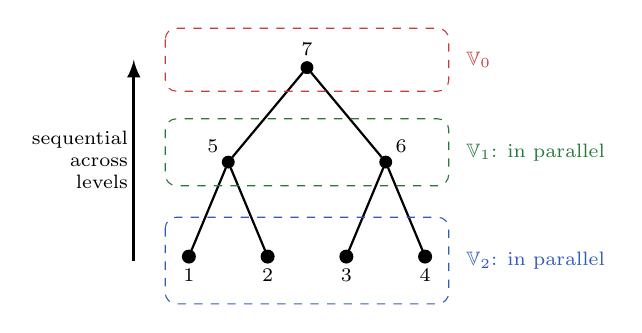
\begin{tikzpicture}[
  level distance=12mm,
  level 1/.style={sibling distance=20mm},
  level 2/.style={sibling distance=10mm},
  every node/.style={circle,draw,fill=black,inner sep=1.5pt},
  edge from parent/.style={draw,thick}]
\node (n7) {}
  child { node (n5) {} child { node (n1) {} } child { node (n2) {} } }
  child { node (n6) {} child { node (n3) {} } child { node (n4) {} } };
\begin{scope}[every node/.style={font=\scriptsize}]
\node[above=1pt] at (n7) {$7$};
\node[above left=0pt] at (n5) {$5$};
\node[above right=0pt] at (n6) {$6$};
\foreach \k in {1,2,3,4} \node[below=1pt] at (n\k) {$\k$};
\end{scope}
\draw[lvlzero,dashed,rounded corners] (-18mm,5mm) rectangle (18mm,-3mm);
\draw[lvlone,dashed,rounded corners] (-18mm,-6.5mm) rectangle (18mm,-15mm);
\draw[lvltwo,dashed,rounded corners] (-18mm,-19mm) rectangle (18mm,-30mm);
% parallel within each level
\begin{scope}[every node/.style={anchor=west,font=\scriptsize}]
\node[lvlzero] at (19mm,1mm)     {$\mathbb{V}_0$};
\node[lvlone]  at (19mm,-10.75mm) {$\mathbb{V}_1$: in parallel};
\node[lvltwo]  at (19mm,-24.5mm)  {$\mathbb{V}_2$: in parallel};
\end{scope}
% sequential across levels
\draw[-latex,very thick] (-22mm,-24.5mm) -- (-22mm,1mm)
  node[midway,left,rectangle,draw=none,fill=none,font=\scriptsize,align=right]
  {sequential\\across\\levels};
\end{tikzpicture}
\end{column}

\begin{column}{0.45\textwidth}
\small
These observations are the foundation of the \textbf{implicit ULV solver for TQS}:

\vspace{3mm}
\begin{itemize}
\setlength{\itemsep}{3mm}
\item \textbf{Outer level:} a \emph{sequential} recursion over the levels,
  as in SQS.
\item \textbf{Within each level:} a \emph{parallel} recursion over the nodes,
  as in HSS.
\end{itemize}
\end{column}
\end{columns}

\vspace{6mm}
\begin{block}{Next}
We illustrate the idea on the level-2 regular binary TQS matrix.
\end{block}
\end{frame}

\begin{frame}{Step 1a: compress the leaf block rows (left)}
\begin{columns}[c]
\begin{column}{0.38\textwidth}
\centering
\leafstep{1}

\vspace{2mm}
\scriptsize after $\operatorname{diag}(q_1\ct,q_2\ct,q_3\ct,q_4\ct,I,I,I)$ \\[1mm]
\swatch{nz} unchanged \quad \swatch{mod} modified \quad \swatch{white} zero
\end{column}

\begin{column}{0.60\textwidth}
\footnotesize
Assume square partitions, $m_i=n_i$. Start at the deepest level $\mathbb{V}_2=\{1,2,3,4\}$.

\vspace{2mm}
\textbf{Observation.} For a leaf $i\in\mathbb{V}_2$, every off-diagonal block in block row $i$
\emph{starts} with $\mathrm{Q}^i_{\mathcal{P}(i)}$, e.g.\ row $1$:
\[
\mathrm{Q}^1_5\mathrm{V}^5_{1,2}\mathrm{B}^2_5,\quad
\mathrm{Q}^1_5\mathrm{P}^5_1,\quad
\mathrm{Q}^1_5\mathrm{W}^5_{1,7}\mathrm{P}^7_5,\ \dots
\]
and every off-diagonal block in block column $i$ \emph{ends} with $\mathrm{B}^i_{\mathcal{P}(i)}$.

\vspace{2mm}
\textbf{Compress.} If $\rho_{\mathcal{P}(i),i}<m_i$, compute for each leaf, \emph{in parallel},
a QL factorization with $q_i$ unitary:
\[
q_i\ct\,\mathrm{Q}^i_{\mathcal{P}(i)}=
\begin{bmatrix} 0 \\ \hat{\mathrm{Q}}^i_{\mathcal{P}(i)} \end{bmatrix}
\begin{matrix}\}\,m_i-\rho_{\mathcal{P}(i),i}\\ \}\,\rho_{\mathcal{P}(i),i}\phantom{-m_i}\end{matrix}
\]
Multiplying block row $i$ by $q_i\ct$ zeros the top $m_i-\rho_{\mathcal{P}(i),i}$ rows
outside the diagonal block.
\end{column}
\end{columns}
\end{frame}

\begin{frame}{Step 1b: triangularize the leaf diagonal blocks (right)}
\begin{columns}[c]
\begin{column}{0.38\textwidth}
\centering
\leafstep{2}

\vspace{2mm}
\scriptsize after $\operatorname{diag}(w_1\ct,w_2\ct,w_3\ct,w_4\ct,I,I,I)$ \\[1mm]
\swatch{nz} unchanged \quad \swatch{mod} modified \quad \swatch{white} zero \\[1mm]
\tikz\fill[tri] (0,0) -- (0,2mm) -- (2mm,0) -- cycle; lower-triangular $\mathrm{D}^i_{11}$
\end{column}

\begin{column}{0.60\textwidth}
\footnotesize
\textbf{Triangularize.} For each leaf $i\in\mathbb{V}_2$, \emph{in parallel}, an LQ factorization
with $w_i$ unitary:
\[
\bigl(q_i\ct\mathrm{D}^i\bigr)\,w_i\ct=
\begin{bmatrix} \mathrm{D}^i_{11} & 0 \\ \mathrm{D}^i_{21} & \mathrm{D}^i_{22} \end{bmatrix},
\qquad \mathrm{D}^i_{11}\ \text{lower triangular}.
\]
Multiply block column $i$ by $w_i\ct$. By the observation, the only other change in
column $i$ is
\[
\mathrm{B}^i_{\mathcal{P}(i)}\,w_i\ct=
\begin{bmatrix} \breve{\mathrm{B}}^i_{\mathcal{P}(i)} & \hat{\mathrm{B}}^i_{\mathcal{P}(i)} \end{bmatrix},
\]
split as the columns of $\mathrm{D}^i$: $m_i-\rho_{\mathcal{P}(i),i}$ and $\rho_{\mathcal{P}(i),i}$.

\vspace{2mm}
\textbf{Result.} $\operatorname{diag}(q_i\ct)\,\mathrm{T}\,\operatorname{diag}(w_i\ct)$ is again a TQS matrix
on the same tree. Only the leaf generators changed:
\begin{gather*}
\mathrm{D}^i \to \begin{bmatrix} \mathrm{D}^i_{11} & 0 \\ \mathrm{D}^i_{21} & \mathrm{D}^i_{22} \end{bmatrix},\qquad
\mathrm{Q}^i_{\mathcal{P}(i)} \to \begin{bmatrix} 0 \\ \hat{\mathrm{Q}}^i_{\mathcal{P}(i)} \end{bmatrix},\\
\mathrm{B}^i_{\mathcal{P}(i)} \to \begin{bmatrix} \breve{\mathrm{B}}^i_{\mathcal{P}(i)} & \hat{\mathrm{B}}^i_{\mathcal{P}(i)} \end{bmatrix},
\qquad \text{all other generators unchanged.}
\end{gather*}
\end{column}
\end{columns}
\end{frame}

\begin{frame}{Step 1c: solve for the $z_i$ (in parallel)}
\begin{columns}[c]
\begin{column}{0.44\textwidth}
\centering
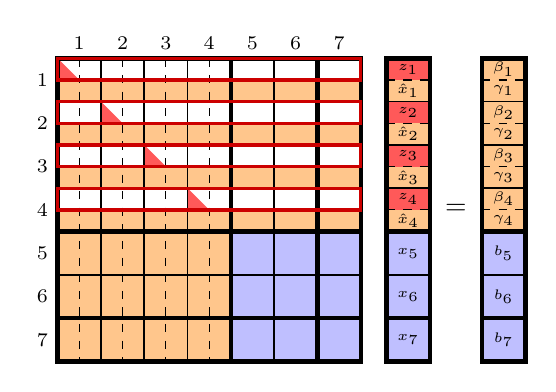
\begin{tikzpicture}[x=5.5mm,y=-5.5mm]
\leafpattern{2}
% the solved rows: top part of each leaf block row
\foreach \i in {1,...,4} \draw[red!80!black,very thick] (0,\i-1) rectangle (7,\i-0.5);
% unknowns w_i x_i and right-hand side q_i^H b_i
\begin{scope}[xshift=7.6*5.5mm]
\fill[nz] (0,0) rectangle (1,7); \fill[mod] (0,0) rectangle (1,4);
\foreach \i in {1,...,4} {\fill[tri] (0,\i-1) rectangle (1,\i-0.5);
  \node[font=\tiny] at (0.5,\i-0.75) {$z_\i$}; \node[font=\tiny] at (0.5,\i-0.25) {$\hat{x}_\i$};}
\foreach \i in {5,6,7} \node[font=\tiny] at (0.5,\i-0.5) {$x_\i$};
\foreach \k in {1,...,6} \draw[line width=0.6pt] (0,\k) -- (1,\k);
\foreach \i in {1,...,4} \draw[dashed,line width=0.4pt] (0,\i-0.5) -- (1,\i-0.5);
\draw[line width=1.6pt] (0,0) rectangle (1,7) (0,4) -- (1,4) (0,6) -- (1,6);
\end{scope}
\node at (9.2,3.5) {$=$};
\begin{scope}[xshift=9.8*5.5mm]
\fill[nz] (0,0) rectangle (1,7); \fill[mod] (0,0) rectangle (1,4);
\foreach \i in {1,...,4} {\node[font=\tiny] at (0.5,\i-0.75) {$\beta_\i$};
  \node[font=\tiny] at (0.5,\i-0.25) {$\gamma_\i$};}
\foreach \i in {5,6,7} \node[font=\tiny] at (0.5,\i-0.5) {$b_\i$};
\foreach \k in {1,...,6} \draw[line width=0.6pt] (0,\k) -- (1,\k);
\foreach \i in {1,...,4} \draw[dashed,line width=0.4pt] (0,\i-0.5) -- (1,\i-0.5);
\draw[line width=1.6pt] (0,0) rectangle (1,7) (0,4) -- (1,4) (0,6) -- (1,6);
\end{scope}
\end{tikzpicture}

\vspace{2mm}
\scriptsize
\tikz\draw[red!80!black,very thick] (0,0) rectangle (4mm,2mm); rows solved in this step \quad
\swatch{tri} $z_i$, now known
\end{column}

\begin{column}{0.54\textwidth}
\footnotesize
Apply the same transformations to the system $\mathrm{T}x=b$:
\[
\bigl(\operatorname{diag}(q_i\ct)\,\mathrm{T}\,\operatorname{diag}(w_i\ct)\bigr)\,
\bigl(\operatorname{diag}(w_i)\,x\bigr)=\operatorname{diag}(q_i\ct)\,b,
\]
with $q_i=w_i=I$ for the nodes $5,6,7$. For each leaf $i\in\mathbb{V}_2$ split
\[
w_i x_i=\begin{bmatrix} z_i \\ \hat{x}_i \end{bmatrix},\qquad
q_i\ct b_i=\begin{bmatrix} \beta_i \\ \gamma_i \end{bmatrix}
\begin{matrix}\}\,m_i-\rho_{\mathcal{P}(i),i}\\ \}\,\rho_{\mathcal{P}(i),i}\phantom{-m_i}\end{matrix}
\]

\vspace{1mm}
The top $m_i-\rho_{\mathcal{P}(i),i}$ rows of block row $i$ are zero outside the diagonal
block, where they read $[\,\mathrm{D}^i_{11}\ \ 0\,]$. Hence
\[
\mathrm{D}^i_{11}\,z_i=\beta_i,\qquad i=1,2,3,4:
\]
four independent lower-triangular solves, done \emph{in parallel}.

\vspace{1mm}
Still unknown: $\hat{x}_1,\dots,\hat{x}_4$ and $x_5,x_6,x_7$.
\end{column}
\end{columns}
\end{frame}

\begin{frame}{Step 1d: move the $z_i$ to the right-hand side and deflate}
\begin{columns}[c]
\begin{column}{0.40\textwidth}
\centering
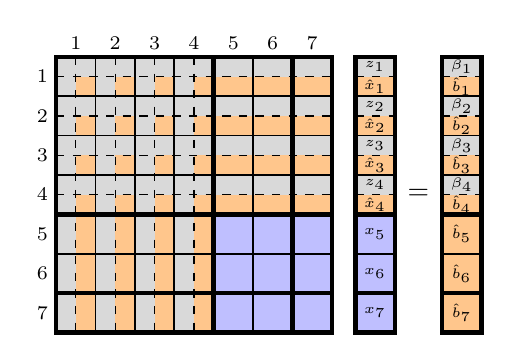
\begin{tikzpicture}[x=5mm,y=-5mm]
\leafpattern{3}
\begin{scope}[xshift=7.6*5mm]
\fill[mod] (0,0) rectangle (1,4); \fill[nz] (0,4) rectangle (1,7);
\foreach \i in {1,...,4} {\fill[gone] (0,\i-1) rectangle (1,\i-0.5);
  \node[font=\tiny] at (0.5,\i-0.75) {$z_\i$}; \node[font=\tiny] at (0.5,\i-0.25) {$\hat{x}_\i$};}
\foreach \i in {5,6,7} \node[font=\tiny] at (0.5,\i-0.5) {$x_\i$};
\foreach \k in {1,...,6} \draw[line width=0.6pt] (0,\k) -- (1,\k);
\foreach \i in {1,...,4} \draw[dashed,line width=0.4pt] (0,\i-0.5) -- (1,\i-0.5);
\draw[line width=1.6pt] (0,0) rectangle (1,7) (0,4) -- (1,4) (0,6) -- (1,6);
\end{scope}
\node at (9.2,3.5) {$=$};
\begin{scope}[xshift=9.8*5mm]
\fill[mod] (0,0) rectangle (1,7);
\foreach \i in {1,...,4} {\fill[gone] (0,\i-1) rectangle (1,\i-0.5);
  \node[font=\tiny] at (0.5,\i-0.75) {$\beta_\i$}; \node[font=\tiny] at (0.5,\i-0.25) {$\hat{b}_\i$};}
\foreach \i in {5,6,7} \node[font=\tiny] at (0.5,\i-0.5) {$\hat{b}_\i$};
\foreach \k in {1,...,6} \draw[line width=0.6pt] (0,\k) -- (1,\k);
\foreach \i in {1,...,4} \draw[dashed,line width=0.4pt] (0,\i-0.5) -- (1,\i-0.5);
\draw[line width=1.6pt] (0,0) rectangle (1,7) (0,4) -- (1,4) (0,6) -- (1,6);
\end{scope}
\end{tikzpicture}

\vspace{2mm}
\scriptsize
\swatch{gone} deflated \quad \swatch{mod} modified \quad \swatch{nz} unchanged
\end{column}

\begin{column}{0.58\textwidth}
\footnotesize
\textbf{Right-hand side.} Every off-diagonal block in column $j$ ends with
$\mathrm{B}^j_{\mathcal{P}(j)}w_j\ct$, so the known $z_j$ enters the other rows only through
\[
g_j=\breve{\mathrm{B}}^j_{\mathcal{P}(j)}\,z_j,\qquad j=1,2,3,4.
\]
For example,
\begin{align*}
\hat{b}_5&=b_5-\mathrm{C}^5_1g_1-\mathrm{C}^5_2g_2-\mathrm{Q}^5_7\mathrm{V}^7_{5,6}\bigl(\mathrm{U}^6_{7,3}g_3+\mathrm{U}^6_{7,4}g_4\bigr),\\
\hat{b}_1&=\gamma_1-\mathrm{D}^1_{21}z_1-\hat{\mathrm{Q}}^1_5\bigl[\mathrm{V}^5_{1,2}g_2
  +\mathrm{W}^5_{1,7}\mathrm{V}^7_{5,6}\bigl(\mathrm{U}^6_{7,3}g_3+\mathrm{U}^6_{7,4}g_4\bigr)\bigr].
\end{align*}
All updates together are one TQS matrix--vector product with inputs $g_j$ at the leaves:
one sweep up and one sweep down the tree.

\vspace{1mm}
\textbf{Deflate.} Drop the solved rows and the $z_i$ columns. The remaining system
$\hat{\mathrm{T}}\hat{x}=\hat{b}$ is TQS on the same tree, with leaf generators
$\mathrm{D}^i_{22}$, $\hat{\mathrm{Q}}^i_{\mathcal{P}(i)}$, $\hat{\mathrm{B}}^i_{\mathcal{P}(i)}$;
leaf $i$ is now of size $\rho_{\mathcal{P}(i),i}\times\rho_{\mathcal{P}(i),i}$.
\end{column}
\end{columns}
\end{frame}

\begin{frame}{Step 1e: merge the leaves into their parents}
\begin{columns}[c]
\begin{column}{0.56\textwidth}
\centering
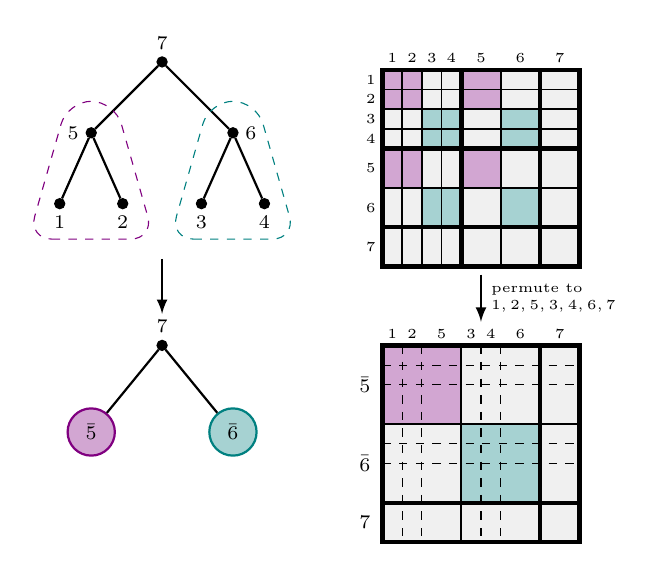
\begin{tikzpicture}[dot/.style={circle,draw,fill=black,inner sep=1.3pt}]
% ---- graph, before
\node[dot] (n7) at (0,0) {};
\node[dot] (n5) at (-9mm,-9mm) {};   \node[dot] (n6) at (9mm,-9mm) {};
\node[dot] (n1) at (-13mm,-18mm) {}; \node[dot] (n2) at (-5mm,-18mm) {};
\node[dot] (n3) at (5mm,-18mm) {};   \node[dot] (n4) at (13mm,-18mm) {};
\draw[thick] (n7) -- (n5) -- (n1) (n5) -- (n2) (n7) -- (n6) -- (n3) (n6) -- (n4);
\begin{scope}[every node/.style={font=\scriptsize}]
\node[above=1pt] at (n7) {$7$};
\node[left=1pt] at (n5) {$5$}; \node[right=1pt] at (n6) {$6$};
\foreach \k in {1,2,3,4} \node[below=1pt] at (n\k) {$\k$};
\end{scope}
\draw[violet,dashed,rounded corners=3mm] (-17mm,-22.5mm) -- (-1mm,-22.5mm) -- (-6mm,-5mm) -- (-12mm,-5mm) -- cycle;
\draw[teal,dashed,rounded corners=3mm] (1mm,-22.5mm) -- (17mm,-22.5mm) -- (12mm,-5mm) -- (6mm,-5mm) -- cycle;
% ---- graph, after
\draw[-latex,thick] (0,-25mm) -- (0,-32mm);
\node[dot] (m7) at (0,-36mm) {};
\node[circle,draw=violet,fill=grpA,thick,minimum size=6mm,font=\scriptsize] (m5) at (-9mm,-47mm) {$\bar{5}$};
\node[circle,draw=teal,fill=grpB,thick,minimum size=6mm,font=\scriptsize] (m6) at (9mm,-47mm) {$\bar{6}$};
\draw[thick] (m5) -- (m7) -- (m6);
\node[above=1pt,font=\scriptsize] at (m7) {$7$};
% ---- matrix, before (deflated; leaf blocks now half size)
\begin{scope}[shift={(28mm,-1mm)},x=5mm,y=-5mm]
\fill[gray!12] (0,0) rectangle (5,5);
\foreach \r/\ra/\rb/\rg in {1/0/0.5/A,2/0.5/1/A,3/1/1.5/B,4/1.5/2/B,5/2/3/A,6/3/4/B} {
  \foreach \c/\ca/\cb/\cg in {1/0/0.5/A,2/0.5/1/A,3/1/1.5/B,4/1.5/2/B,5/2/3/A,6/3/4/B} {
    \ifx\rg\cg \fill[grp\rg] (\ca,\ra) rectangle (\cb,\rb); \fi}}
\foreach \k in {0.5,1,1.5,3} \draw[line width=0.6pt] (\k,0) -- (\k,5) (0,\k) -- (5,\k);
\draw[line width=1.6pt] (0,0) rectangle (5,5) (2,0) -- (2,5) (4,0) -- (4,5) (0,2) -- (5,2) (0,4) -- (5,4);
\foreach \k/\m in {1/0.25,2/0.75,3/1.25,4/1.75,5/2.5,6/3.5,7/4.5} {
  \node[font=\tiny] at (\m,-0.3) {$\k$}; \node[font=\tiny] at (-0.3,\m) {$\k$};}
\end{scope}
% ---- matrix, after (permuted to 1,2,5 | 3,4,6 | 7)
\draw[-latex,thick] (40.5mm,-27mm) -- node[right,font=\tiny,align=left] {permute to\\$1,2,5,3,4,6,7$} (40.5mm,-33mm);
\begin{scope}[shift={(28mm,-36mm)},x=5mm,y=-5mm]
\fill[gray!12] (0,0) rectangle (5,5);
\fill[grpA] (0,0) rectangle (2,2); \fill[grpB] (2,2) rectangle (4,4);
\foreach \k in {0.5,1,2.5,3} \draw[dashed,line width=0.4pt] (\k,0) -- (\k,5) (0,\k) -- (5,\k);
\draw[line width=0.6pt] (2,0) -- (2,5) (0,2) -- (5,2);
\draw[line width=1.6pt] (0,0) rectangle (5,5) (4,0) -- (4,5) (0,4) -- (5,4);
\foreach \k/\m in {1/0.25,2/0.75,5/1.5,3/2.25,4/2.75,6/3.5} \node[font=\tiny] at (\m,-0.3) {$\k$};
\node[font=\tiny] at (4.5,-0.3) {$7$};
\node[font=\scriptsize] at (-0.45,1) {$\bar{5}$}; \node[font=\scriptsize] at (-0.45,3) {$\bar{6}$};
\node[font=\scriptsize] at (-0.45,4.5) {$7$};
\end{scope}
\end{tikzpicture}
\end{column}

\begin{column}{0.42\textwidth}
\footnotesize
\textbf{No more compression.} After deflation leaf $i$ has $\rho_{\mathcal{P}(i),i}$ rows,
as many as $\hat{\mathrm{Q}}^i_{\mathcal{P}(i)}$ has columns: no zero rows can be created.

\vspace{2mm}
\textbf{Merge.} Every node of $\mathbb{V}_1$ absorbs its children:
\[
\bar{5}=\{1,2,5\},\qquad \bar{6}=\{3,4,6\}.
\]
In the matrix: permute to $1,2,5\,|\,3,4,6\,|\,7$ and regroup the blocks.

\vspace{2mm}
\textbf{Result.} A TQS matrix on the depth-1 tree $7-\{\bar{5},\bar{6}\}$; the states on
the edges between $7$ and $\bar{5},\bar{6}$ are unchanged. E.g.
\[
\mathrm{B}^{\bar{5}}_7=\begin{bmatrix}\mathrm{U}^5_{7,1}\hat{\mathrm{B}}^1_5 & \mathrm{U}^5_{7,2}\hat{\mathrm{B}}^2_5 & \mathrm{B}^5_7\end{bmatrix}.
\]
Next: repeat Step 1 on the new leaves $\bar{5},\bar{6}$.
\end{column}
\end{columns}
\end{frame}

\begin{frame}{Step 2: solve the merged TQS system}
\begin{columns}[c]
\begin{column}{0.46\textwidth}
\centering
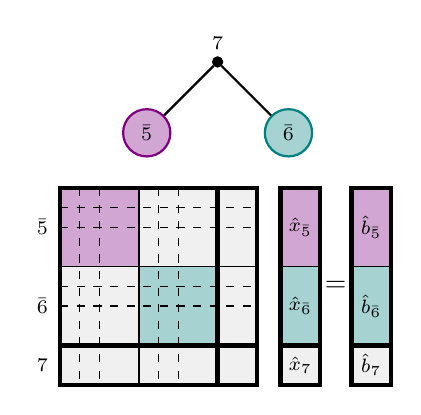
\begin{tikzpicture}[dot/.style={circle,draw,fill=black,inner sep=1.3pt}]
% merged tree
\node[dot] (m7) at (0,0) {};
\node[circle,draw=violet,fill=grpA,thick,minimum size=6mm,font=\scriptsize] (m5) at (-9mm,-9mm) {$\bar{5}$};
\node[circle,draw=teal,fill=grpB,thick,minimum size=6mm,font=\scriptsize] (m6) at (9mm,-9mm) {$\bar{6}$};
\draw[thick] (m5) -- (m7) -- (m6);
\node[above=1pt,font=\scriptsize] at (m7) {$7$};
% merged system  T^ x^ = b^
\begin{scope}[shift={(-20mm,-16mm)},x=5mm,y=-5mm]
\fill[gray!12] (0,0) rectangle (5,5);
\fill[grpA] (0,0) rectangle (2,2); \fill[grpB] (2,2) rectangle (4,4);
\foreach \k in {0.5,1,2.5,3} \draw[dashed,line width=0.4pt] (\k,0) -- (\k,5) (0,\k) -- (5,\k);
\draw[line width=0.6pt] (2,0) -- (2,5) (0,2) -- (5,2);
\draw[line width=1.6pt] (0,0) rectangle (5,5) (4,0) -- (4,5) (0,4) -- (5,4);
\node[font=\scriptsize] at (-0.45,1) {$\bar{5}$}; \node[font=\scriptsize] at (-0.45,3) {$\bar{6}$};
\node[font=\scriptsize] at (-0.45,4.5) {$7$};
% unknowns and right-hand side
\foreach \v/\xs/\nm in {x/5.6/{\hat{x}},b/7.4/{\hat{b}}} {
  \begin{scope}[xshift=\xs*5mm]
  \fill[gray!12] (0,0) rectangle (1,5);
  \fill[grpA] (0,0) rectangle (1,2); \fill[grpB] (0,2) rectangle (1,4);
  \draw[line width=0.6pt] (0,2) -- (1,2);
  \draw[line width=1.6pt] (0,0) rectangle (1,5) (0,4) -- (1,4);
  \node[font=\scriptsize] at (0.5,1) {$\nm_{\bar{5}}$};
  \node[font=\scriptsize] at (0.5,3) {$\nm_{\bar{6}}$};
  \node[font=\scriptsize] at (0.5,4.5) {$\nm_7$};
  \end{scope}}
\node at (7,2.5) {$=$};
\end{scope}
\end{tikzpicture}
\end{column}

\begin{column}{0.52\textwidth}
\footnotesize
The merged system $\hat{\mathrm{T}}\hat{x}=\hat{b}$ is a TQS system on the depth-1 tree, with the
right-hand side $\hat{b}$ from Step 1d. The unknowns are stacked per merged node:
$\hat{x}_{\bar{5}}$ stacks $\hat{x}_1,\hat{x}_2,x_5$; $\hat{x}_{\bar{6}}$ stacks $\hat{x}_3,\hat{x}_4,x_6$;
$\hat{x}_7=x_7$ (likewise for $\hat{b}$).

\vspace{1mm}
Solve it with the \emph{same} steps, now at the leaves $\bar{5},\bar{6}\in\mathbb{V}_1$,
\emph{in parallel}:
\begin{itemize}
\setlength{\itemsep}{0pt}
\item[1a] compress with $\mathrm{Q}^{\bar{5}}_7$, $\mathrm{Q}^{\bar{6}}_7$ (left);
\item[1b] triangularize $\mathrm{D}^{\bar{5}}$, $\mathrm{D}^{\bar{6}}$ (right);
\item[1c] solve for $z_{\bar{5}}$, $z_{\bar{6}}$;
\item[1d] update the right-hand side and deflate;
\item[1e] merge $\bar{5}$, $\bar{6}$ into the root $7$.
\end{itemize}
What remains is a single dense block at the root, solved directly.
\end{column}
\end{columns}

\vspace{1mm}
\begin{block}{Recursive property}
The level-2 TQS system is reduced to solving a level-1 TQS problem.
\end{block}
\end{frame}

\begin{frame}{General problem statement}
\begin{columns}[c]
\begin{column}{0.62\textwidth}
\footnotesize
Let $\mathrm{T}$ be a TQS matrix on a tree $\mathbb{G}$ of depth $L\ge1$ with root $r$ and square
partitions $m_k=n_k$.

\vspace{2mm}
Node $k$ with children $c_1,\dots,c_d$ and parent $a$ has the \emph{spinner matrix}
(rows: outgoing edges and output; columns: incoming edges and input)
\[
\mathrm{S}^k=
\begin{bNiceMatrix}[first-row,first-col]
 & c_1 & \cdots & c_d & a & \text{in} \\
c_1 & 0 & \cdots & \mathrm{V}^k_{c_1,c_d} & \mathrm{W}^k_{c_1,a} & \mathrm{P}^k_{c_1} \\
\vdots & \vdots & \ddots & \vdots & \vdots & \vdots \\
c_d & \mathrm{V}^k_{c_d,c_1} & \cdots & 0 & \mathrm{W}^k_{c_d,a} & \mathrm{P}^k_{c_d} \\
a & \mathrm{U}^k_{a,c_1} & \cdots & \mathrm{U}^k_{a,c_d} & 0 & \mathrm{B}^k_a \\
\text{out} & \mathrm{C}^k_{c_1} & \cdots & \mathrm{C}^k_{c_d} & \mathrm{Q}^k_a & \mathrm{D}^k
\end{bNiceMatrix}.
\]

\vspace{3mm}
\textbf{Problem:} solve
\[
\mathrm{T}x=b.
\]
\end{column}

\begin{column}{0.36\textwidth}
\centering
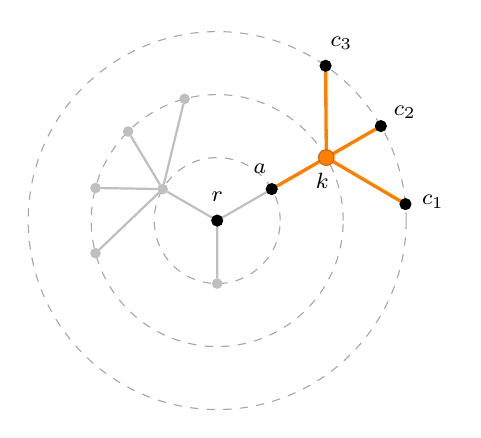
\begin{tikzpicture}[tdot/.style={circle,draw=gray!50,fill=gray!50,inner sep=1.2pt},
                    tedge/.style={thick,gray!50}]
\radialtreebase
% the node k = 9, its children and its parent
\draw[very thick,orange] (n10) -- (n9) (n9) -- (n6) (n9) -- (n7) (n9) -- (n8);
\foreach \k in {10,6,7,8,12} \node[circle,draw,fill=black,inner sep=1.4pt] at (n\k) {};
\node[circle,draw=orange!80!black,fill=orange,inner sep=2pt] at (n9) {};
\begin{scope}[every node/.style={font=\footnotesize}]
\node at ($(n9)+(-100:3mm)$) {$k$};
\node at ($(n10)+(120:3mm)$) {$a$};
\node at ($(n12)+(90:3mm)$) {$r$};
\node at ($(n6)+(5:3.5mm)$) {$c_1$};
\node at ($(n7)+(30:3.5mm)$) {$c_2$};
\node at ($(n8)+(55:3.5mm)$) {$c_3$};
\end{scope}
\end{tikzpicture}

\vspace{2mm}
\scriptsize example: node $k$ with $d=3$ children and parent $a$
\end{column}
\end{columns}

\end{frame}

\begin{frame}{The pruned tree (level-based)}
\footnotesize
\begin{definition}[Pruned tree]
\upshape
Let $\mathbb{G}=(\mathbb{V},\mathbb{E})$ be a tree with root $r$, depth $L\ge1$ and levels
$\mathbb{V}_0,\dots,\mathbb{V}_L$. For $p\in\mathbb{V}_{L-1}$ define the \emph{merged node}
$\bar{p}:=\{p\}\cup\mathcal{C}(p)$, and let $\pi(p)=\bar{p}$ for $p\in\mathbb{V}_{L-1}$, $\pi(k)=k$ otherwise.
The \emph{pruned tree} $\tilde{\mathbb{G}}=(\tilde{\mathbb{V}},\tilde{\mathbb{E}})$ is
\[
\tilde{\mathbb{V}}=\mathbb{V}_0\cup\dots\cup\mathbb{V}_{L-2}\cup\{\bar{p}:p\in\mathbb{V}_{L-1}\},\qquad
\tilde{\mathbb{E}}=\{(\pi(i),\pi(j)) : (i,j)\in\mathbb{E},\ i,j\notin\mathbb{V}_L\}.
\]
It has root $\pi(r)$, depth $L-1$, levels $\tilde{\mathbb{V}}_\ell=\mathbb{V}_\ell$ for $\ell\le L-2$ and
$\tilde{\mathbb{V}}_{L-1}=\{\bar{p}:p\in\mathbb{V}_{L-1}\}$; every $\bar{p}$ is a leaf.
\end{definition}

\centering
% the notation-slide tree rerooted at its center 10 (AST slide): levels on circles of radius 8l mm
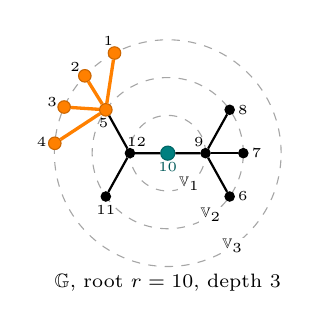
\begin{tikzpicture}[baseline=(n10.center),scale=0.6,
  dot/.style={circle,draw,fill=black,inner sep=1.2pt},
  hot/.style={circle,draw=orange!80!black,fill=orange,inner sep=1.6pt},
  root/.style={circle,draw=teal!80!black,fill=teal,inner sep=1.8pt}]
\foreach \r in {8,16,24} \draw[gray!70,dashed] (0,0) circle (\r mm);
\node[root] (n10) at (0,0) {};
\node[dot] (n12) at (180:8mm) {}; \node[dot] (n9) at (0:8mm) {};
\node[hot] (n5) at (145:16mm) {}; \node[dot] (n11) at (215:16mm) {};
\foreach \k/\a in {6/-35,7/0,8/35} \node[dot] (n\k) at (\a:16mm) {};
\foreach \k/\a in {1/118,2/137,3/156,4/175} \node[hot] (n\k) at (\a:24mm) {};
\draw[thick] (n10) -- (n12) (n10) -- (n9) (n12) -- (n11) (n12) -- (n5);
\foreach \k in {6,7,8} \draw[thick] (n9) -- (n\k);
\draw[very thick,orange] \foreach \k in {1,2,3,4} {(n5) -- (n\k)};
\foreach \k/\a in {12/60,9/120,5/260,11/270,6/0,7/0,8/0,1/118,2/137,3/156,4/175}
  \node[font=\tiny] at ($(n\k)+(\a:2.8mm)$) {$\k$};
\node[font=\tiny,teal!70!black] at ($(n10)+(270:3mm)$) {$10$};
\foreach \l/\r in {1/8,2/16,3/24}
  \node[font=\tiny,fill=white,inner sep=0.5pt] at (-55:\r mm) {$\mathbb{V}_\l$};
\node[font=\scriptsize] at (0,-27.5mm) {$\mathbb{G}$, root $r=10$, depth $3$};
\end{tikzpicture}
\hspace{4mm}
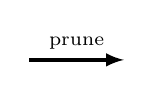
\begin{tikzpicture}[baseline=(c.center)]
\coordinate (c) at (0,0);
\draw[-latex,very thick] (0,0) -- node[above,font=\scriptsize] {prune} (12mm,0);
\end{tikzpicture}
\hspace{4mm}
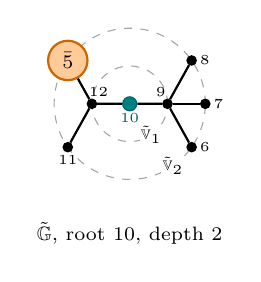
\begin{tikzpicture}[baseline=(n10.center),scale=0.6,
  dot/.style={circle,draw,fill=black,inner sep=1.2pt},
  root/.style={circle,draw=teal!80!black,fill=teal,inner sep=1.8pt}]
\foreach \r in {8,16} \draw[gray!70,dashed] (0,0) circle (\r mm);
\node[root] (n10) at (0,0) {};
\node[dot] (n12) at (180:8mm) {}; \node[dot] (n9) at (0:8mm) {};
\node[circle,draw=orange!80!black,fill=orange!40,thick,minimum size=5mm,inner sep=0pt,font=\scriptsize]
  (n5) at (145:16mm) {$\bar{5}$};
\node[dot] (n11) at (215:16mm) {};
\foreach \k/\a in {6/-35,7/0,8/35} \node[dot] (n\k) at (\a:16mm) {};
\draw[thick] (n10) -- (n12) (n10) -- (n9) (n12) -- (n11) (n12) -- (n5);
\foreach \k in {6,7,8} \draw[thick] (n9) -- (n\k);
\foreach \k/\a in {12/60,9/120,11/270,6/0,7/0,8/0}
  \node[font=\tiny] at ($(n\k)+(\a:2.8mm)$) {$\k$};
\node[font=\tiny,teal!70!black] at ($(n10)+(270:3mm)$) {$10$};
\foreach \l/\r in {1/8,2/16}
  \node[font=\tiny,fill=white,inner sep=0.5pt] at (-55:\r mm) {$\tilde{\mathbb{V}}_\l$};
\node[font=\scriptsize,align=center] at (0,-27.5mm) {$\tilde{\mathbb{G}}$, root $10$, depth $2$};
\end{tikzpicture}

\scriptsize Root $10$ (teal), the center of the tree; why this root is chosen comes later. Only the deepest level $\mathbb{V}_3=\{1,2,3,4\}$ is pruned: $\bar{5}=\{5,1,2,3,4\}$.
The leaves $11,6,7,8\in\mathbb{V}_2$ wait for the next round.
\end{frame}

\begin{frame}{Leaf operations}
\footnotesize
For every leaf $i\in\mathbb{V}_L$, \emph{in parallel}, with parent $p=\mathcal{P}(i)$, set
$k_i:=\max(m_i-\rho_{p,i},0)$ (rows that can be compressed) and $\hat{m}_i:=m_i-k_i$.

\vspace{2mm}
\centering
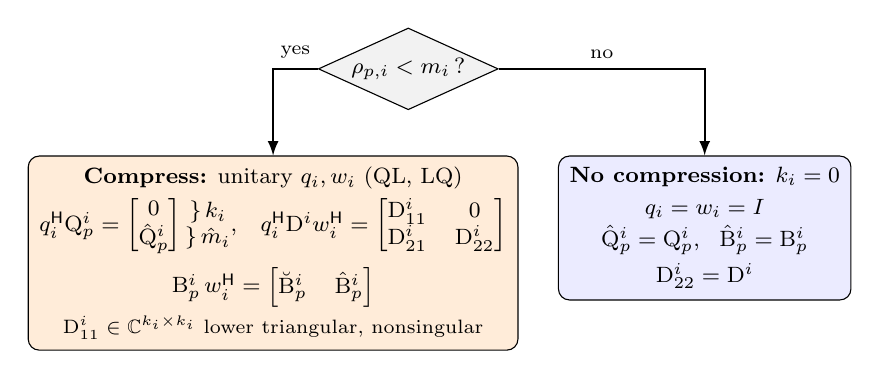
\begin{tikzpicture}[
  box/.style={draw,rounded corners,align=center,inner sep=4pt,font=\footnotesize},
  flow/.style={-latex,thick},
  lbl/.style={font=\scriptsize,midway}]
\node[diamond,draw,aspect=2.2,inner sep=1pt,font=\footnotesize,fill=gray!10] (dec) {$\rho_{p,i}<m_i$\,?};
\node[box,fill=orange!15,anchor=north east] (yes) at (14mm,-11mm) {%
  \textbf{Compress:} unitary $q_i,w_i$ (QL, LQ)\\[2pt]
  $q_i\ct\mathrm{Q}^i_p=\begin{bmatrix}0\\ \hat{\mathrm{Q}}^i_p\end{bmatrix}
   \begin{matrix}\}\,k_i\\ \}\,\hat{m}_i\end{matrix}$,\quad
  $q_i\ct\mathrm{D}^iw_i\ct=\begin{bmatrix}\mathrm{D}^i_{11}&0\\ \mathrm{D}^i_{21}&\mathrm{D}^i_{22}\end{bmatrix}$\\[4pt]
  $\mathrm{B}^i_p\,w_i\ct=\begin{bmatrix}\breve{\mathrm{B}}^i_p & \hat{\mathrm{B}}^i_p\end{bmatrix}$\\[2pt]
  {\scriptsize $\mathrm{D}^i_{11}\in\mathbb{C}^{k_i\times k_i}$ lower triangular, nonsingular}};
\node[box,fill=blue!8,anchor=north west] (no) at (19mm,-11mm) {%
  \textbf{No compression:} $k_i=0$\\[2pt]
  $q_i=w_i=I$\\[2pt]
  $\hat{\mathrm{Q}}^i_p=\mathrm{Q}^i_p,\ \ \hat{\mathrm{B}}^i_p=\mathrm{B}^i_p$\\[2pt]
  $\mathrm{D}^i_{22}=\mathrm{D}^i$};
\draw[flow] (dec.west) -| node[lbl,above,pos=0.25] {yes} (yes.north);
\draw[flow] (dec.east) -| node[lbl,above,pos=0.25] {no} (no.north);
\end{tikzpicture}

\vspace{2mm}
\raggedright
\textbf{Local variables,} split as $k_i$ and $\hat{m}_i$ ($z_i$, $\beta_i$ empty if $k_i=0$):
\[
w_ix_i=\begin{bmatrix} z_i \\ \hat{x}_i \end{bmatrix},\qquad
q_i\ct b_i=\begin{bmatrix} \beta_i \\ \gamma_i \end{bmatrix}.
\]
\end{frame}

\begin{frame}{The reduced TQS matrix}
\footnotesize
\begin{definition}[Reduced TQS matrix]
\upshape
$\tilde{\mathrm{T}}$ is the TQS matrix on the pruned tree $\tilde{\mathbb{G}}$ with the same edge states
$\rho$ and the following spinners.
\begin{itemize}
\setlength{\itemsep}{2mm}
\item \textbf{Higher up in the tree, unchanged:}\quad
  $\tilde{\mathrm{S}}^k=\mathrm{S}^k$ for $k\in\mathbb{V}_0\cup\dots\cup\mathbb{V}_{L-2}$.
\item \textbf{Merged leaves:} for $p\in\mathbb{V}_{L-1}$ with children $c_1,\dots,c_d$ and parent $a$,
  the leaf $\bar{p}$ has size $m_p+\sum_{j=1}^{d}\hat{m}_{c_j}$ and spinner\footnote{If $p=r$, then $\tilde{\mathrm{S}}^{\bar{p}}=\tilde{\mathrm{D}}^{\bar{p}}$.}
\end{itemize}
\[
\tilde{\mathrm{S}}^{\bar{p}}=\begin{bmatrix}0 & \tilde{\mathrm{B}}^{\bar{p}}_a\\ \tilde{\mathrm{Q}}^{\bar{p}}_a & \tilde{\mathrm{D}}^{\bar{p}}\end{bmatrix},\qquad
\tilde{\mathrm{D}}^{\bar{p}}=\begin{bmatrix}
\mathrm{D}^{c_1}_{22} & \cdots & \hat{\mathrm{Q}}^{c_1}_p\mathrm{V}^p_{c_1,c_d}\hat{\mathrm{B}}^{c_d}_p & \hat{\mathrm{Q}}^{c_1}_p\mathrm{P}^p_{c_1}\\
\vdots & \ddots & \vdots & \vdots\\
\hat{\mathrm{Q}}^{c_d}_p\mathrm{V}^p_{c_d,c_1}\hat{\mathrm{B}}^{c_1}_p & \cdots & \mathrm{D}^{c_d}_{22} & \hat{\mathrm{Q}}^{c_d}_p\mathrm{P}^p_{c_d}\\
\mathrm{C}^p_{c_1}\hat{\mathrm{B}}^{c_1}_p & \cdots & \mathrm{C}^p_{c_d}\hat{\mathrm{B}}^{c_d}_p & \mathrm{D}^p
\end{bmatrix},
\]
\[
\tilde{\mathrm{Q}}^{\bar{p}}_a=\begin{bmatrix}\hat{\mathrm{Q}}^{c_1}_p\mathrm{W}^p_{c_1,a}\\ \vdots\\ \hat{\mathrm{Q}}^{c_d}_p\mathrm{W}^p_{c_d,a}\\ \mathrm{Q}^p_a\end{bmatrix},\qquad
\tilde{\mathrm{B}}^{\bar{p}}_a=\begin{bmatrix}\mathrm{U}^p_{a,c_1}\hat{\mathrm{B}}^{c_1}_p & \cdots & \mathrm{U}^p_{a,c_d}\hat{\mathrm{B}}^{c_d}_p & \mathrm{B}^p_a\end{bmatrix}.
\]
\end{definition}
\end{frame}

\begin{frame}{The reduced unknown}
\footnotesize
\begin{definition}[Reduced unknown]
\upshape
For every merged leaf $\bar{p}$, $p\in\mathbb{V}_{L-1}$ with children $c_1,\dots,c_d$: transform each child,
$w_{c_j}x_{c_j}=\left[\begin{smallmatrix}z_{c_j}\\ \hat{x}_{c_j}\end{smallmatrix}\right]$, keep the remaining part
$\hat{x}_{c_j}$ and stack it on top of $x_p$:
\[
\tilde{x}_{\bar{p}}=\bigl[\hat{x}_{c_1};\dots;\hat{x}_{c_d};x_p\bigr].
\]
All other nodes keep their unknown: $\tilde{x}_k=x_k$ for $k\in\mathbb{V}_0\cup\dots\cup\mathbb{V}_{L-2}$.
\end{definition}

\centering
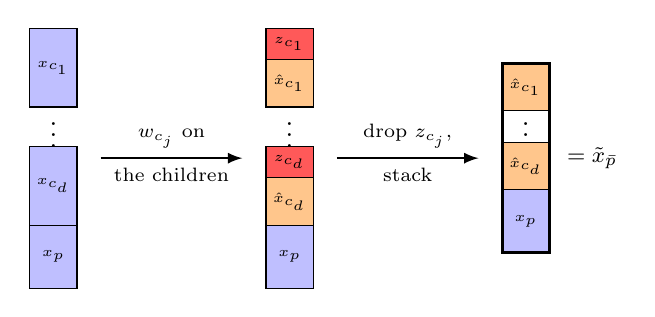
\begin{tikzpicture}
% original unknowns of the nodes c_1, ..., c_d, p
\vblk{0mm}{0mm}{10mm}{nz}{$x_{c_1}$}
\node at (3mm,-12.5mm) {$\vdots$};
\vblk{0mm}{-15mm}{10mm}{nz}{$x_{c_d}$}
\vblk{0mm}{-25mm}{8mm}{nz}{$x_p$}
\draw[-latex,thick] (9mm,-16.5mm) -- node[above,font=\scriptsize] {$w_{c_j}$ on} node[below,font=\scriptsize] {the children} (27mm,-16.5mm);
% transformed: z (red) on top of x-hat (orange)
\vblk{30mm}{0mm}{4mm}{tri}{$z_{c_1}$}  \vblk{30mm}{-4mm}{6mm}{mod}{$\hat{x}_{c_1}$}
\node at (33mm,-12.5mm) {$\vdots$};
\vblk{30mm}{-15mm}{4mm}{tri}{$z_{c_d}$} \vblk{30mm}{-19mm}{6mm}{mod}{$\hat{x}_{c_d}$}
\vblk{30mm}{-25mm}{8mm}{nz}{$x_p$}
\draw[-latex,thick] (39mm,-16.5mm) -- node[above,font=\scriptsize] {drop $z_{c_j}$,} node[below,font=\scriptsize] {stack} (57mm,-16.5mm);
% reduced unknown of the merged leaf
\vblk{60mm}{-4.5mm}{6mm}{mod}{$\hat{x}_{c_1}$}
\node at (63mm,-12.5mm) {$\vdots$};
\vblk{60mm}{-14.5mm}{6mm}{mod}{$\hat{x}_{c_d}$}
\vblk{60mm}{-20.5mm}{8mm}{nz}{$x_p$}
\draw[very thick] (60mm,-4.5mm) rectangle (66mm,-28.5mm);
\node[right,font=\footnotesize] at (67mm,-16.5mm) {$=\tilde{x}_{\bar{p}}$};
\end{tikzpicture}

\vspace{1mm}
\scriptsize
\swatch{nz} unchanged \quad \swatch{mod} kept, transformed \quad \swatch{tri} $z_{c_j}$, fixed by $z_{c_j}=(\mathrm{D}^{c_j}_{11})^{-1}\beta_{c_j}$
\end{frame}

\begin{frame}{The reduced right-hand side}
\footnotesize
\begin{definition}[Reduced right-hand side]
\upshape
Every leaf $j\in\mathbb{V}_L$ sends the known state $g_j:=\breve{\mathrm{B}}^j_{\mathcal{P}(j)}z_j$ into its edge
$(j,\mathcal{P}(j))$. With the path transition $\Phi_{k,j}$ and $p_{\nu-1}$ the last node before $k$ on the path from $j$,
\[
\hat{b}_i=\gamma_i-\mathrm{D}^i_{21}z_i-\sum_{j\in\mathbb{V}_L\setminus\{i\}}\hat{\mathrm{Q}}^i_{\mathcal{P}(i)}\,
  \Phi_{i,j}\,g_j\quad(i\in\mathbb{V}_L),
\qquad
\hat{b}_k=b_k-\sum_{j\in\mathbb{V}_L}\mathrm{Out}^k_{p_{\nu-1}}\,
  \Phi_{k,j}\,g_j\quad(k\notin\mathbb{V}_L).
\]
Stack as the unknown: $\tilde{b}_{\bar{p}}=\bigl[\hat{b}_{c_1};\dots;\hat{b}_{c_d};\hat{b}_p\bigr]$, and $\tilde{b}_k=\hat{b}_k$ otherwise.
\end{definition}

\begin{columns}[c]
\begin{column}{0.5\textwidth}
\scriptsize
$\Phi_{k,j}$ carries $g_j$ along the unique path from $j$ to $k$; $\mathrm{Out}^k_{p_{\nu-1}}$ ($\mathrm{C}$ or $\mathrm{Q}$)
reads it out at $k$. The paths share their transitions ($\Phi_{k,j}=\Phi_{k,l}\Phi_{l,j}$ for $l$ on the path):
one sweep up and one sweep down the tree carries the $g_j$ to every node.
\end{column}
\begin{column}{0.48\textwidth}
\centering
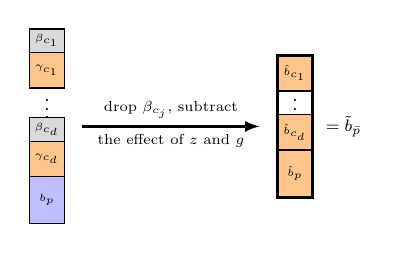
\begin{tikzpicture}[scale=0.75,every node/.style={transform shape}]
% q^H b on the children, b on p
\vblk{0mm}{0mm}{4mm}{gone}{$\beta_{c_1}$}  \vblk{0mm}{-4mm}{6mm}{mod}{$\gamma_{c_1}$}
\node at (3mm,-12.5mm) {$\vdots$};
\vblk{0mm}{-15mm}{4mm}{gone}{$\beta_{c_d}$} \vblk{0mm}{-19mm}{6mm}{mod}{$\gamma_{c_d}$}
\vblk{0mm}{-25mm}{8mm}{nz}{$b_p$}
\draw[-latex,thick] (9mm,-16.5mm) -- node[above,font=\scriptsize] {drop $\beta_{c_j}$, subtract} node[below,font=\scriptsize] {the effect of $z$ and $g$} (39mm,-16.5mm);
% reduced right-hand side of the merged leaf
\vblk{42mm}{-4.5mm}{6mm}{mod}{$\hat{b}_{c_1}$}
\node at (45mm,-12.5mm) {$\vdots$};
\vblk{42mm}{-14.5mm}{6mm}{mod}{$\hat{b}_{c_d}$}
\vblk{42mm}{-20.5mm}{8mm}{mod}{$\hat{b}_p$}
\draw[very thick] (42mm,-4.5mm) rectangle (48mm,-28.5mm);
\node[right,font=\footnotesize] at (49mm,-16.5mm) {$=\tilde{b}_{\bar{p}}$};
\end{tikzpicture}
\end{column}
\end{columns}
\end{frame}

\begin{frame}{The reduction theorem}
\small
\begin{theorem}
\upshape
Let $\tilde{\mathrm{T}}$, $\tilde{x}$ and $\tilde{b}$ be the reduced TQS matrix, unknown and right-hand side.
Then $x$ solves $\mathrm{T}x=b$ if and only if
\[
z_i=(\mathrm{D}^i_{11})^{-1}\beta_i\quad(i\in\mathbb{V}_L)
\qquad\text{and}\qquad
\tilde{\mathrm{T}}\tilde{x}=\tilde{b}.
\]
The solution is recovered as $x_i=w_i\ct\begin{bmatrix}z_i\\ \hat{x}_i\end{bmatrix}$ for $i\in\mathbb{V}_L$.
\end{theorem}
\end{frame}

\begin{frame}{The recursive solver (level-based)}
\footnotesize
Applying the reduction theorem until the tree is a single node gives Algorithm~\ref{alg:tqssolve}.

\begin{algorithm}[H]
\scriptsize
\caption{\footnotesize Implicit ULV solve of a TQS system $\mathrm{T}x=b$}
\label{alg:tqssolve}
\begin{algorithmic}[1]
\Function{TQSSolve}{$\mathrm{T}$, $\mathbb{G}$, $b$}\Comment{$\mathbb{G}$ of depth $L$}
  \If{$L=0$}
    \State \Return $x_r=(\mathrm{D}^r)^{-1}b_r$\Comment{one dense solve at the root}
  \EndIf
  \ForAll{$i\in\mathbb{V}_L$ \textbf{in parallel}}
    \State leaf operations: $q_i,w_i$, $\hat{\mathrm{Q}}^i_p$, $\hat{\mathrm{B}}^i_p$, $\mathrm{D}^i_{22}$;\ \
      $\left[\begin{smallmatrix}\beta_i\\ \gamma_i\end{smallmatrix}\right]=q_i\ct b_i$
    \State $z_i\gets(\mathrm{D}^i_{11})^{-1}\beta_i$\Comment{lower-triangular solve}
  \EndFor
  \State form $\tilde{b}$ from $g_j=\breve{\mathrm{B}}^j_{\mathcal{P}(j)}z_j$\Comment{one sweep up and down the tree}
  \State form $\tilde{\mathrm{T}}$ on the pruned tree $\tilde{\mathbb{G}}$\Comment{merge spinners, in parallel over $\mathbb{V}_{L-1}$}
  \State $\tilde{x}\gets\Call{TQSSolve}{\tilde{\mathrm{T}},\tilde{\mathbb{G}},\tilde{b}}$\Comment{depth $L-1$}
  \State unstack $\tilde{x}_{\bar{p}}=[\hat{x}_{c_1};\dots;\hat{x}_{c_d};x_p]$, and
    $x_i\gets w_i\ct\left[\begin{smallmatrix}z_i\\ \hat{x}_i\end{smallmatrix}\right]$ for $i\in\mathbb{V}_L$
  \State \Return $x$
\EndFunction
\end{algorithmic}
\end{algorithm}

$L+1$ sequential rounds (SQS-like, across the levels); within a round all leaves are independent (HSS-like).
\end{frame}

\begin{frame}{Special cases: SSS and HSS}
\footnotesize
SSS and HSS matrices are TQS matrices on special trees (Section~3.4 of the original paper). On these trees
Algorithm~\ref{alg:tqssolve} reduces to the known implicit ULV solvers (orange: current leaves, teal: root).

\vspace{2mm}
\begin{columns}[T]
\begin{column}{0.48\textwidth}
\textbf{SSS: line graph}

\centering
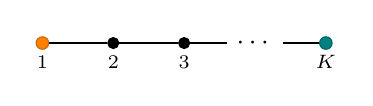
\begin{tikzpicture}[dot/.style={circle,draw,fill=black,inner sep=1.4pt}]
\foreach \k/\xx in {1/9,2/18,3/27} \node[dot] (s\k) at (\xx mm,0) {};
\node (sd) at (36mm,0) {$\cdots$};
\node[circle,draw=teal!80!black,fill=teal,inner sep=1.6pt] (sK) at (45mm,0) {};
\draw[thick] (s1) -- (s2) -- (s3) -- (sd) -- (sK);
\node[circle,draw=orange!80!black,fill=orange,inner sep=1.6pt] at (s1) {};
\foreach \k in {1,2,3} \node[below=1pt,font=\scriptsize] at (s\k) {$\k$};
\node[below=1pt,font=\scriptsize] at (sK) {$K$};
\end{tikzpicture}

\raggedright
\scriptsize
Root $r=K$: $L=K-1$, one node per level.
\begin{itemize}\setlength{\itemsep}{0pt}
\item each round has a single leaf: compress it, solve for its $z$, merge it into the next node
  (first round: leaf $1$, $\bar{2}=\{2,1\}$);
\item $K$ sequential rounds, no parallelism within a round;
\item this is the implicit ULV solver for SSS~[1,2].
\end{itemize}
Rooting at the middle instead (see onion peeling, later): both ends in parallel, ${\approx}K/2$ rounds.
\end{column}
\begin{column}{0.48\textwidth}
\textbf{HSS: binary tree, virtual non-leaf nodes}

\centering
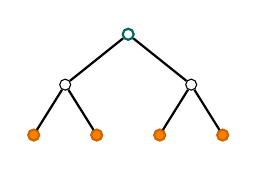
\begin{tikzpicture}[scale=0.8,
  level distance=8mm,
  level 1/.style={sibling distance=20mm},
  level 2/.style={sibling distance=10mm},
  every node/.style={circle,draw,fill=white,inner sep=1.4pt},
  edge from parent/.style={draw,thick}]
\node[draw=teal!80!black,fill=white,thick] {}
  child { node {} child { node[fill=orange,draw=orange!80!black] {} } child { node[fill=orange,draw=orange!80!black] {} } }
  child { node {} child { node[fill=orange,draw=orange!80!black] {} } child { node[fill=orange,draw=orange!80!black] {} } };
\end{tikzpicture}

\raggedright
\scriptsize
Non-leaf nodes are virtual ($m_k=n_k=0$, open circles), so $x_p$ and $b_p$ are empty.
\begin{itemize}\setlength{\itemsep}{0pt}
\item each round compresses all leaves in parallel and merges sibling pairs: $\tilde{\mathrm{D}}^{\bar{p}}$ is the
  $2\times2$ block of the reduced children;
\item the root solve is the base case;
\item this is the implicit ULV solver for HSS~[3].
\end{itemize}
\end{column}
\end{columns}

\vfill
\raggedright
\tiny
[1] S.~Chandrasekaran, P.~Dewilde, M.~Gu, T.~Pals, A.-J.~van der Veen, \emph{Fast stable solver for sequentially semi-separable linear systems of equations}, HiPC 2002, 545--554.\par
[2] S.~Chandrasekaran, P.~Dewilde, M.~Gu, T.~Pals, X.~Sun, A.-J.~van der Veen, D.~White, \emph{Some fast algorithms for sequentially semiseparable representations}, SIAM J.\ Matrix Anal.\ Appl.\ 27(2), 2005, 341--364.\par
[3] S.~Chandrasekaran, M.~Gu, T.~Pals, \emph{A fast ULV decomposition solver for hierarchically semiseparable representations}, SIAM J.\ Matrix Anal.\ Appl.\ 28(3), 2006, 603--622.
\end{frame}

\begin{frame}{Complexity: regular binary tree}
\footnotesize
\textbf{Assumptions.} Regular binary tree with $K$ nodes, all blocks $m_k=n_k=n$ and all states
$\rho_{i,j}=\rho$. Matrix size $N=Kn$. Let $\mathcal{T}(K)$ be the cost of \textsc{TQSSolve} on such a tree.

\textbf{Leaf sizes stay bounded:} a leaf keeps $\hat{m}\le\rho$ rows, so a merged leaf $\{p,c_1,c_2\}$ has size $s\le n+2\rho$.

\textbf{Work in one call} (excluding the recursive call), with $(K+1)/2$ leaves:
\begin{center}
\scriptsize
\renewcommand{\arraystretch}{1.1}
\begin{tabular}{@{}lll@{}}
\hline
step & per leaf / node & per call \\
\hline
QL, LQ, column update & $O(s^3)$ & $O\bigl(K(n+\rho)^3\bigr)$ \\
triangular solve for $z_i$ & $O(s^2)$ & $O\bigl(K(n+\rho)^2\bigr)$ \\
right-hand side: sweep with the $g_j$ & $O\bigl((n+\rho)^2\bigr)$ & $O\bigl(K(n+\rho)^2\bigr)$ \\
merge spinners & $O\bigl((n+\rho)\,\rho^2\bigr)$ & $O\bigl(K(n+\rho)\,\rho^2\bigr)$ \\
\hline
\end{tabular}
\end{center}

\textbf{Recurrence.} The pruned tree has $(K-1)/2$ nodes; the base case is one dense solve of size $\le n+2\rho$:
\[
\mathcal{T}(K)=\mathcal{T}(K/2)+\Theta\bigl(K(n+\rho)^3\bigr),\qquad \mathcal{T}(1)=\Theta\bigl((n+\rho)^3\bigr).
\]
\textbf{Master theorem} with $a=1$, $b=2$, $f(K)=\Theta(K(n+\rho)^3)$: since $\log_b a=0<1$ and
$a\,f(K/b)=\tfrac12 f(K)$, case 3 applies:
\[
\mathcal{T}(K)=\Theta\bigl(f(K)\bigr)=\Theta\bigl(K(n+\rho)^3\bigr)=\Theta\!\left(N\,\frac{(n+\rho)^3}{n}\right),
\]
i.e.\ linear in $N$ for fixed $n,\rho$.
\end{frame}

\begin{frame}{Applicative single token pass (AST) model: maximizing parallelism}
\footnotesize
Which root should we pick? Algorithm~\ref{alg:tqssolve} works level by level, from the deepest level to the root:
$L+1$ \emph{sequential} rounds, $L$ the depth of the rooted tree. So the root should not be picked
arbitrarily: choose it to minimize the depth.

\vspace{1mm}
\textbf{Onion peeling.} Repeatedly remove \emph{all} current leaves at once. This ends with a single node or two adjacent
nodes, the \emph{center} of the tree; take it (either of the two) as root. Then $L$ equals the radius of the tree,
the smallest possible depth.

\vspace{2mm}
\centering
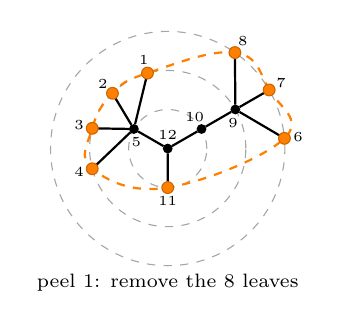
\begin{tikzpicture}[scale=0.62,tdot/.style={circle,draw,fill=black,inner sep=1.1pt},tedge/.style={thick}]
\radialtreebase
% one dashed curve through the nodes peeled in this round
\draw[orange,dashed,thick] plot[smooth cycle,tension=0.7] coordinates {(n6) (n7) (n8) (n1) (n2) (n3) (n4) (n11)};
\foreach \k in {1,2,3,4,6,7,8,11} \node[circle,draw=orange!80!black,fill=orange,inner sep=1.5pt] at (n\k) {};
\foreach \k/\a in {12/90,5/280,10/120,11/270,9/-100,1/105,2/135,3/165,4/195,6/5,7/30,8/55}
  \node[font=\tiny] at ($(n\k)+(\a:2.8mm)$) {$\k$};
\node[font=\scriptsize] at (0,-27.5mm) {peel 1: remove the $8$ leaves};
\end{tikzpicture}
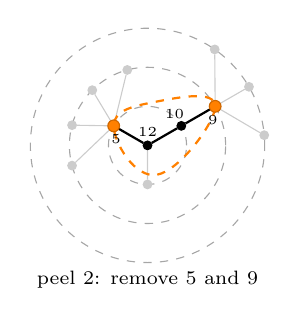
\begin{tikzpicture}[scale=0.62,tdot/.style={circle,draw=gray!40,fill=gray!40,inner sep=1.1pt},tedge/.style={gray!40}]
\radialtreebase
\draw[thick] (n5) -- (n12) -- (n10) -- (n9);
\foreach \k in {12,10} \node[circle,draw,fill=black,inner sep=1.1pt] at (n\k) {};
\draw[orange,dashed,thick] plot[smooth cycle,tension=0.8] coordinates {(n5) (2mm,-6mm) (n9) (2mm,9mm)};
\foreach \k in {5,9} \node[circle,draw=orange!80!black,fill=orange,inner sep=1.5pt] at (n\k) {};
\foreach \k/\a in {12/90,5/280,10/120,9/-100} \node[font=\tiny] at ($(n\k)+(\a:2.8mm)$) {$\k$};
\node[font=\scriptsize] at (0,-27.5mm) {peel 2: remove $5$ and $9$};
\end{tikzpicture}
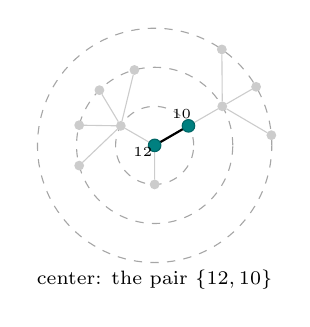
\begin{tikzpicture}[scale=0.62,tdot/.style={circle,draw=gray!40,fill=gray!40,inner sep=1.1pt},tedge/.style={gray!40}]
\radialtreebase
\draw[thick] (n12) -- (n10);
\foreach \k in {12,10} \node[circle,draw=teal!80!black,fill=teal,inner sep=1.6pt] at (n\k) {};
\foreach \k/\a in {12/210,10/120} \node[font=\tiny] at ($(n\k)+(\a:2.8mm)$) {$\k$};
\node[font=\scriptsize] at (0,-27.5mm) {center: the pair $\{12,10\}$};
\end{tikzpicture}

\vspace{1mm}
\raggedright
\textbf{Example.} Root $12$ (as in the notation slide) or $10$: depth $L=3$, i.e.\ $4$ rounds, which is optimal.
A poor choice, e.g.\ the leaf $6$ as root, gives depth $5$, i.e.\ $6$ rounds, with fewer nodes per level to process in parallel.
\end{frame}

\begin{frame}{AST pruning: prune all leaves at once}
\footnotesize
Level-based pruning removes only the deepest level $\mathbb{V}_L$; a leaf higher up waits until its level is the deepest.
\emph{AST pruning} removes all leaves in every round, as in onion peeling.

\begin{definition}[AST-pruned tree]
\upshape
Let $\mathbb{L}:=\{i\neq r:\mathcal{C}(i)=\emptyset\}$ be the set of \emph{all} leaves of $\mathbb{G}$. For every $p$ with
at least one leaf child, split its children into the leaf children $c_1,\dots,c_d\in\mathbb{L}$ and the remaining children
$e_1,\dots,e_f\notin\mathbb{L}$, and set $\bar{p}:=\{p,c_1,\dots,c_d\}$. With $\pi(p)=\bar{p}$ for these $p$ and
$\pi(k)=k$ otherwise, the AST-pruned tree $\tilde{\mathbb{G}}$ has
\[
\tilde{\mathbb{V}}=\{\pi(k):k\notin\mathbb{L}\},\qquad
\tilde{\mathbb{E}}=\{(\pi(i),\pi(j)) : (i,j)\in\mathbb{E},\ i,j\notin\mathbb{L}\},
\]
and the same root $\pi(r)$.
\end{definition}

\vspace{1mm}
Two differences with the level-based version:
\begin{itemize}
\item leaves at different depths are pruned in the same round;
\item $\bar{p}$ need not be a leaf of $\tilde{\mathbb{G}}$: it keeps its remaining children $e_1,\dots,e_f$.
\end{itemize}
The leaf operations, the reduced unknown and right-hand side, the reduction theorem and
Algorithm~\ref{alg:tqssolve} hold verbatim with $\mathbb{V}_L$ replaced by $\mathbb{L}$. Only the spinner of $\bar{p}$
gains blocks for the edges to $e_1,\dots,e_f$ (next slide).
\end{frame}

\begin{frame}{AST pruning: spinner of a merged node}
\footnotesize
Let $p$ have leaf children $c_1,\dots,c_d$, remaining children $e_1,\dots,e_f$ and parent $a$. The merged node $\bar{p}$ has

\vspace{2mm}
\begin{columns}[T]
\begin{column}{0.5\textwidth}
\[
\tilde{\mathrm{S}}^{\bar{p}}=
\begin{bNiceMatrix}[first-row,first-col]
 & e_1 & \cdots & e_f & a & \text{in} \\
e_1 & 0 & \cdots & \mathrm{V}^p_{e_1,e_f} & \mathrm{W}^p_{e_1,a} & \tilde{\mathrm{P}}^{\bar{p}}_{e_1} \\
\vdots & \vdots & \ddots & \vdots & \vdots & \vdots \\
e_f & \mathrm{V}^p_{e_f,e_1} & \cdots & 0 & \mathrm{W}^p_{e_f,a} & \tilde{\mathrm{P}}^{\bar{p}}_{e_f} \\
a & \mathrm{U}^p_{a,e_1} & \cdots & \mathrm{U}^p_{a,e_f} & 0 & \tilde{\mathrm{B}}^{\bar{p}}_a \\
\text{out} & \tilde{\mathrm{C}}^{\bar{p}}_{e_1} & \cdots & \tilde{\mathrm{C}}^{\bar{p}}_{e_f} & \tilde{\mathrm{Q}}^{\bar{p}}_a & \tilde{\mathrm{D}}^{\bar{p}}
\end{bNiceMatrix}
\]
\end{column}
\begin{column}{0.48\textwidth}
$\tilde{\mathrm{D}}^{\bar{p}}$, $\tilde{\mathrm{Q}}^{\bar{p}}_a$, $\tilde{\mathrm{B}}^{\bar{p}}_a$: as in the level-based case. For each remaining child $e$:
\[
\tilde{\mathrm{P}}^{\bar{p}}_{e}=\begin{bmatrix}\mathrm{V}^p_{e,c_1}\hat{\mathrm{B}}^{c_1}_p & \cdots & \mathrm{V}^p_{e,c_d}\hat{\mathrm{B}}^{c_d}_p & \mathrm{P}^p_{e}\end{bmatrix},
\]
\[
\tilde{\mathrm{C}}^{\bar{p}}_{e}=\begin{bmatrix}\hat{\mathrm{Q}}^{c_1}_p\mathrm{V}^p_{c_1,e}\\ \vdots\\ \hat{\mathrm{Q}}^{c_d}_p\mathrm{V}^p_{c_d,e}\\ \mathrm{C}^p_{e}\end{bmatrix}.
\]
\end{column}
\end{columns}

\scriptsize
\begin{itemize}\setlength{\itemsep}{0pt}
\item Paths between two remaining neighbours of $\bar{p}$ do not touch the leaves: transitions unchanged.
\item Paths from or to the leaf $c_j$ pick up $\hat{\mathrm{B}}^{c_j}_p$ or $\hat{\mathrm{Q}}^{c_j}_p$ and the child-to-child transition $\mathrm{V}^p$.
\item If $f=0$ this is the level-based spinner; if $p=r$, drop the row and column $a$. Every other node keeps $\tilde{\mathrm{S}}^k=\mathrm{S}^k$.
\end{itemize}
\end{frame}

\begin{frame}{Level-based versus AST pruning: example}
\footnotesize
\begin{columns}[c]
\begin{column}{0.3\textwidth}
\centering
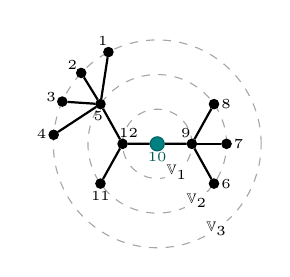
\begin{tikzpicture}[scale=0.55,
  dot/.style={circle,draw,fill=black,inner sep=1.2pt},
  root/.style={circle,draw=teal!80!black,fill=teal,inner sep=1.8pt}]
\foreach \r in {8,16,24} \draw[gray!70,dashed] (0,0) circle (\r mm);
\node[root] (n10) at (0,0) {};
\node[dot] (n12) at (180:8mm) {}; \node[dot] (n9) at (0:8mm) {};
\node[dot] (n5) at (145:16mm) {}; \node[dot] (n11) at (215:16mm) {};
\foreach \k/\a in {6/-35,7/0,8/35} \node[dot] (n\k) at (\a:16mm) {};
\foreach \k/\a in {1/118,2/137,3/156,4/175} \node[dot] (n\k) at (\a:24mm) {};
\draw[thick] (n10) -- (n12) (n10) -- (n9) (n12) -- (n11) (n12) -- (n5);
\foreach \k in {6,7,8} \draw[thick] (n9) -- (n\k);
\foreach \k in {1,2,3,4} \draw[thick] (n5) -- (n\k);
\foreach \k/\a in {12/60,9/120,5/260,11/270,6/0,7/0,8/0,1/118,2/137,3/156,4/175}
  \node[font=\tiny] at ($(n\k)+(\a:2.8mm)$) {$\k$};
\node[font=\tiny,teal!70!black] at ($(n10)+(270:3mm)$) {$10$};
\foreach \l/\r in {1/8,2/16,3/24}
  \node[font=\tiny,fill=white,inner sep=0.5pt] at (-55:\r mm) {$\mathbb{V}_\l$};
\end{tikzpicture}

\scriptsize root $r=10$, depth $L=3$
\end{column}
\begin{column}{0.68\textwidth}
\scriptsize
\renewcommand{\arraystretch}{1.35}
\setlength{\tabcolsep}{4pt}
\begin{tabular}{@{}l>{\raggedright\arraybackslash}p{0.36\linewidth}>{\raggedright\arraybackslash}p{0.36\linewidth}@{}}
\hline
\textbf{Round} & \textbf{Level-based}: prune $\mathbb{V}_L$ & \textbf{AST}: prune $\mathbb{L}$ \\
\hline
1 & $1,2,3,4\to5$ & $1,2,3,4\to5$;\ $11\to12$;\newline $6,7,8\to9$ \\
2 & $\bar{5},11\to12$;\ $6,7,8\to9$ & $\bar{5}\to\bar{12}$;\ $\bar{9}\to10$ \\
3 & $\bar{12},\bar{9}\to10$ & $\bar{12}\to\bar{10}$ \\
4 & dense solve at $\bar{10}$ & dense solve at $\bar{10}$ \\
\hline
leaves/round & $4,\ 5,\ 2$ & $8,\ 2,\ 1$ \\
\hline
\end{tabular}

\vspace{1mm}
$i\to p$: leaf $i$ is compressed and merged into its parent $p$; a bar marks a merged node.
\end{column}
\end{columns}

\vspace{3mm}
\begin{itemize}
\item \textbf{Same number of rounds} for a fixed root: $k\in\mathbb{V}_\ell$ is pruned in round $L+1-\ell$ (level-based, as late as possible)
  or in round $h(k)+1$ (AST, as soon as possible), with $h(k)$ the length of the longest path from $k$ down to a leaf. Both end in round $L+1$.
\item \textbf{AST front-loads the work}: more leaves in parallel early on, and the tree shrinks faster.
\item \textbf{AST needs no root}: peeling all degree-one nodes is onion peeling, so it ends at the center by itself.
\end{itemize}
\end{frame}

\begin{frame}{Pending tasks}
\footnotesize
\begin{itemize}
\setlength{\itemsep}{3mm}
\item \textbf{Implementation and experiments.} Implement the solver and run experiments: study the
  complexity and the memory consumption.
\item \textbf{Explicit factorization.} Compute an explicit factorization
  $\mathrm{T}=\mathcal{U}\mathcal{L}\mathcal{V}$ ($\mathcal{U},\mathcal{V}$ unitary, $\mathcal{L}$ lower triangular)
  with $\mathcal{U},\mathcal{L},\mathcal{V}$ in structured representation. Important for multiple right-hand sides:
  factor once, solve many times.
\item \textbf{Applications.} Exterior Helmholtz equation on a branchy domain; boundary value problems on cracks?
\item \textbf{Side-gig: optimality of TQS.} For the example of Section~3.5 of the original paper
  (sparse matrices whose adjacency graph is a regular binary tree), prove that the TQS representation is the most compact:
  for \emph{no} ordering of the nodes of $\mathrm{T}$ does a pure HSS or SSS representation of $\mathrm{T}$ become more compact.
\end{itemize}
\end{frame}

\end{document}
